% !TeX program = pdflatex
\documentclass[11pt]{report} 
\usepackage{minted}
\usepackage[utf8]{inputenc}
\usepackage{amssymb}
\usepackage{xcolor}
\usepackage{listings}
\usepackage{xparse}
	\usepackage{xspace}
\usepackage{placeins}
\usepackage[english]{babel}
\usepackage{amsmath}
\usepackage{caption}
\usepackage[T1]{fontenc}
\usepackage{amsfonts}

\usepackage{tocloft}
\setlength{\cftsecindent}{0em}
\setlength{\cftsubsecindent}{0em}
\setlength{\cftsubsubsecindent}{0em}

\renewcommand{\cftsecfont}{\normalfont\bfseries}% titles in bold
\renewcommand{\cftsecpagefont}{\normalfont\bfseries}% page numbers in bold
\renewcommand{\cftdotsep}{1}
\renewcommand{\cftsecleader}{\bfseries\cftdotfill{\cftsecdotsep}}% dot leaders in bold
\usepackage{tikz}
\usetikzlibrary{automata, positioning, arrows, matrix}
\tikzset{
	->,
	>=stealth,
	node distance=3cm,
	align=center,
	every state/.style={thick, fill=gray!10},
	initial text=$ $
}
\lstset{
	frameround=fttt,
	language=C,
	numbers=left,basewidth=0.5em,
	breaklines=true,
	basicstyle=\ttfamily\color{blue},
	columns=fixed,
	numberstyle=\color{maroon},
}
	
%\usepackage{geometry}
%\usepackage{natbib}
\usepackage{textcomp}
\usepackage[scaled=.81]{beramono}
\usepackage[sc]{mathpazo} % add possibly `sc` and `osf` options
\usepackage{eulervm}
\usepackage[Lenny]{fncychap}
\usepackage{soul}
\setlength{\headheight}{15pt}
\usepackage[llbracket]{stmaryrd}
\setcounter{tocdepth}{6}
\setcounter{secnumdepth}{6}
\usepackage{amsthm}
\usepackage{url}
\usepackage{verbatim}
\usepackage{graphicx}
\usepackage{algorithm}
%\usepackage[noend]{algpseudocode}
%\usepackage{qtree}
%\usepackage{subfig}
%\usepackage{mathpartir}
\usepackage{dirtree}
\setminted{
	fontsize=\footnotesize{},
	linenos,
	tabsize=2,
	breaklines,
	frame=lines,
	samepage=true
}

\newcommand{\code}[1]{\textcolor{blue}{\texttt{#1}}}
\newcommand{\gapwedge}{\ \wedge{}\ }
\newcommand{\ruledef}[4]{
	#1 & \texttt{#3} & $\rightarrow{}$ & \texttt{#4} & #2 \\
}
\captionsetup{width=.9\linewidth}
\newtheorem{assumption}{Assumption}
\usepackage{booktabs}
\usepackage{titlesec}
\usepackage{fancyhdr}
\pagestyle{fancy}

\titleformat{\section}
{\Large\bfseries\rm}
  {\thesection}{1em}{}
  
\titleformat{\subsection}
{\large\bfseries\rm}
  {\thesubsection}{1em}{}

\captionsetup{width=.9\linewidth}



\fancyhf{}
\lhead{}
\rhead{\rightmark}
\cfoot{\thepage}

\definecolor{dblue}{rgb}{0.1,0.2,0.6}
\usepackage[linktocpage=true]{hyperref}
\hypersetup{colorlinks,linkcolor={dblue}, citecolor={dblue},urlcolor={BrickRed}}  

\usepackage{epigraph}
\renewcommand{\epigraphsize}{\small}

\setlength{\epigraphwidth}{0.66\textwidth}
\renewcommand{\textflush}{flushright} \renewcommand{\sourceflush}{flushright}
\newcommand{\Imp}{\Longrightarrow}
\newcommand{\All}{\bigwedge}


\title{Formalizing the Semantics of Concurrent Revisions}
\author{Christopher Esterhuyse}
\date{\today}

\begin{document}

\begin{titlepage}
	\centering
	\includegraphics[width=0.22\textwidth, trim={0 0.15cm 0 0}, clip]{img/vu.png}
%	 \hspace{1.3cm}
%	\includegraphics[width=0.15\textwidth, trim={0 0.74cm 0 0}, clip]{img/uva.eps}
	\par
%	\vspace{1cm}
	{\scshape\huge Vrije Universiteit Amsterdam \par}
	\vspace{1.5cm}
	{\scshape\LARGE Master's thesis\par \par
	\vspace{0.2cm}
	\small \textit{Submitted in partial fulfillment of the requirements for\\ the degree of Master of Science in\\ Parallel and Distributed Computer Systems.}\par}
	\vspace{1.5cm}
	{\Huge\bfseries \rm \textbf{I don't yet know what to call it, lol}\par}
	\vspace{1.5cm}
	{\Large\itshape\rm \noindent\textit{Christopher Esterhuyse}\\}
	\vspace{1mm}
	\textit{(ID: 2553295)}
	\vfill
		\rm \noindent \textit{supervisors} \\ \vspace{0.15cm}
	\begin{tabular}{r@{\hskip 0.4in}l}
\rm \textbf{Vrije Universiteit Amsterdam} & \textbf{Centrum Wiskunde \& Informatica} \\
dr.\ J.\ \textsc{Endrullis} & dr.\ F.\ \textsc{Arbab}
\end{tabular}
\begin{comment}
	\vfill
	\rm supervised by\par
	dr.\ J.C.\ \textsc{Blanchette} (VU), first supervisor \par
	prof. dr.\ W.J.\ \textsc{Fokkink} (VU), second supervisor \par
	ir. R. \textsc{Van Dalen} (ING), daily supervisor
	\end{comment}
	\vfill

% TODO!! check for everyone's honorifics

% Bottom of the page
	{\large \today\par}
\end{titlepage}

\abstract{
TODO
}

\include{parts/preface}

\tableofcontents

\listoffigures

\listoflistings
\listoftables

\newpage

% chapters

\part{Preliminaries}
\chapter{Introduction}
Traditional, sequential programming has been changing for decades. Over time, languages acquired more and more tools to manage the level of abstraction, such that programs were of higher quality, and with a lower cost to develop~\cite{shaw1984abstraction}. This trend continues to this day. For example, conventionally imperative languages such as Java and C++ have since added functional features, such as closures, to capitalize on their brevity and lack of side-effects. 

By comparison, concurrent programming has fallen behind. Although some strides have been made, it is not uncommon for modern programs to dip down to the level of channels, mutex locks and semaphores, which have remained unchanged for decades. As a consequence, large concurrent programs require arcane knowledge, inhibiting the employability of programmers, and retaining the brittleness and obfuscation common to the programs of their day~\cite{chamberlain2007parallel}. This deficiency has not gone unnoticed, and many academic and industrial projects have sought to fill the void. Paradigms such as the \textit{actor model}, various \textit{process calculi} and more have emerged, each offering their take on the right approach to managing abstraction. Farhad et al.\ observed that despite their innovation, such approaches inherited a vestige of their connection to the world of sequential programming: \textit{action-centricism}, ie.\ making explicit the individual actions contributing to interactions, rather than the interaction itself. Although many modern approaches introduce valuable abstractions, they often have in common that they still relegate interactions to a derived concept~\cite{arbab2011puff}. In such programs, the burden is on the programmer to conceptualize the program's runtime behavior to reconstruct these interactions to understand the `big picture'. As programs grow large, these actions become far-flung and interact in complex and unexpected ways. Needless to say, such programs are difficult to reason about, and costly and error-prone in their maintenance.

Reo is an exogenous coordination language developed at the CWI in Amsterdam. The language is designed around the representation of \textit{protocols} which specify the communication between actors as a first-class concept. Reo protocol specifications are dense, self-contained, and declarative, so that it can be easily understood and manipulated by humans and machines alike. Protocols are understood as \textit{relations} between actors, specifying how data is allowed to `flow' between abstract \textit{ports}, each of which send and receive values through the system, oblivious of the protocol and which other ports exist. The idea is to separate (often sequential) \textit{computation work} into weakly-coupled modules, with Reo defining their \textit{communication} only~\cite{arbab2004reo}. With this approach, protocols and compute-components become swappable, re-usable modules; each can be more easily understood, maintained and re-used. The Reo language is designed such that the protocols behave as expected when \textit{composed}; one can reason about components in isolation, safe in the knowledge that their properties are preserved in the system at large. An ecosystem of tooling has sprung up around the Reo language to make use of these explicit protocol specifications, ranging from visualization to verification. 

In this work, we focus on Reo's use in \textit{code generation}. Instead of writing and maintaining an action-centric codebase, programmers are able to write computation code in their language of choice, with \textit{components} independently sending and receiving data through opaque port objects, whose communication is defined separately as a Reo protocol. The \textit{Reo compiler} generates the action-centric glue code as if they programmer had written it themselves, with the guarantee that it behaves as specified~\cite{jongmans2013modularizing}. In this manner, programmers are able to understand and manipulate their code given the best of both worlds: a high-level view into abstract and modular components, while compiled and executed using the language of their choice. Over time, the Reo compiler has been extended to support various compilation-target languages, with Java seeing the most extensive development. 

In this work, we extend the Reo compiler's repertoire of supported language targets by designing and implementing a Rust back-end. Chapter~\ref{sec:imperative_form} describes how this translation is performed. Rust is a favourable choice, as it is easily inter-operable with C and C++, and has a strict type system that allows us to expose an API that guarantees conformance with Reo's intuitive value-passing semantics. Chapter~\ref{sec:protocol_runtime} explains how we are able to leverage Reo's explicit protocols in combination with Rust's systems-level resource management to safely implement various optimizations, such as transparent \textit{reference-passing} for components coordinating in shared-memory. Chapter~\ref{sec:api} investigates leveraging Rust's \textit{affine type system} to offer an ergonomic mechanism to inject \textit{liveness properties} of our Reo-coordinated Rust programs by checking our compute-code for \textit{protocol adherence} at compile time without significant overhead at runtime.



\chapter{Background}
\section{Reo}
\label{sec:reo_background}
Reo is a high-level language for specifying protocols. Here, we explore the motivation behind Reo's development, how the language is used, and (at high level) how it works. 
The Reo language has applicability whenever there is a benefit in being able to formalize a communication protocol. However, this work primarily focuses on Reo's role in automatic generation of glue-code for applications.  

\subsection{Motivation}
\label{sec:reo_motivation}
TODO focus on safety properties

Modern software development involves the construction of large and complex projects. Owing to their scale and the heterogeneity of the tasks required, many people are involved in the development of a program at once, and over its development lifetime. The industry has long-since established paradigms for managing the scale of these projects. One tenet of good software design is \textit{modularity}, which describes a structure that, instead of being designed monolithically, is built out of smaller constituent modules. In addition to isolating modules such that they can be re-used in other projects, this design philosophy allows contributors to concentrate on a subset of all the modules at a time. These ideas are well-established in practice; code re-use and separation-of-concerns have been prevalent for some time.

Reo's utility is not only its ability to facilitate modularity. Reo is designed such that properties of the individual modules are \textit{preserved} when modules are \textit{composed} into larger ones. This preservation marks the difference between \textit{gluing} modules together (and hoping for the best), and \textit{composing} them into something guaranteed to have the intended properties. 

\subsection{Language}
\label{sec:reo_lang}
Reo is a \textit{coordination} language. This describes its focus on the specification of the \textit{interactions} between distinct actors. This is in contrast to the usual \textit{action-centric} model common to languages with their roots in sequential programming, where the programs or specifications describe \textit{actions} of entities, relegating any associated interactions to requiring derivation from the actions. In a nutshell, Reo provides a language for describing the behavior of a \textit{system} of actors by explicitly constraining the behavior of the \textit{connector} which serves as their communication medium. 

(TODO define connector. same as component just maybe structural?)

The Reo language is essentially graphic; each connector defines a relation over named \textit{locations}. Complex connectors are defined as the composition of simpler connectors over its locations. This inherently visual language is also often seen in its textual form, usually in the context of machine parsing. 

The simplest \textit{primitive} connectors cannot be subdivided

by listing a set of constituent connectors. The simplest primitive Reo connectors are \textit{channels}(TODO channel vs primitive). Channels by definition cannot be subdivided into constituent connectors, as they are defined by either (a) the model that provides Reo's semantics, or (b) opaque components defined in some target language such as C or Java. The nodes themselves are the other important aspect of the language. Ultimately, each node corresponds to a (logical) location which may hold up to one datum at a time. Reo is by default \textit{synchronous}, and relationships between locations propagates that synchrony. \textit{Locations} are divided into two classes according to whether 

(TODO)

This motivates the Reo's metaphor of propagation of data and back-propagation of data-constraints, corresponding to its namesake, the Greek word for `flow'. The compositional aspect is meaningful when locations are involved in multiple relationships.

\textit{forwards} (by moving data several `hops' at once) and backwards

In addition to re-using nodes inside a connector, connectors are able to expose these nodes for re-use in the connectors \textit{above them} by exposing the node in the connector's \textit{interface}. These exposed nodes are called \textit{ports}, leaning on the metaphor of the connector \textit{moving} some data in and out of itself.

(data flow corresponds with what happens at runtime, except its SYNCHRONOUS by default. Relate to TDS. Talk about replication and equality checks).

(In the context of applications, components that cannot be composed compile to things managed by different threads. at the boundaries, they communicate with ports. Here, there is a meaningful difference between putter and getter. Include example of how a protocol that uses some port A three times still results in a putter-getter pair)


\subsection{Typical Channels}

In principle, Reo does not enforce the use of any primitive channels in particular. Users are free to use channels that are best-suited to their use case. In practice, a small set of exceptionally simple channels are favoured in literature and in practice owing to their versatility. As such, this work presumes that these consititute the majority of the channels out of which our protocols are composed. Below, we enumerate this set of channels and their behavior.

\begin{enumerate}
	\item sync($I_0, O_0$)
	\item fifo1($I_0, O_0$)
	\item lossy\_sync($I_0, O_0$)
	\item exclusive\_router($I_0, O_0, O_1$)
\end{enumerate}


\subsection{Semantic Models}
\label{sec:semantic_models}
Reo took a number of years to take its present shape. It is recognizable as early as 2001, but was presented as a concept before it was formalized, leaving it as a task for future work~\cite{jongmans2012overview}. Later, This several different approaches to formal semantics were developed. For our purposes, it suffices to concentrate only on the small subset of the semantics to follow. For additional information, the work of Jongmans in particular serves as a good entry point\cite{jongmans2012overview}.


Starting with the fundamentals, a \textbf{stream} specifies the value of a variable from data domain $D$ changing over the course of a sequence of events. Usually streams are considered infinite, and so it is practical to define them as a function $\mathbb{N}\mapsto{}D$. A \textbf{timed data stream} (TDS) takes this notion a step further, annotating each event in the sequence with an increasing \textit{time stamp}. A TDS is defined by some tuple $(\mathbb{N}\mapsto{}\mathbb{R}, \mathbb{N}\mapsto{}D)$, or equivalently, $\mathbb{N}\mapsto{}(\mathbb{R}, D)$ with the added constraints that time must increase toward infinity\cite{arbab2004modeling}. By associating one TDS with each \textit{named variable} of a program, one can represent a \textit{trace} of its execution. TDS events with the same time stamp are considered simultaneous, allowing reasoning about \textit{snapshots} of the program's state over its run time. These traces can be practically visualized as \textbf{trace tables}, with variables for columns and time stamps for rows by representing the absence of data observations using a special `silent' symbol \textbf{*}, referring \textit{silent behavior}. In this work, we use `trace tables' to refer to both the visualization and to a program trace as a set of named TDS's. The runs of finite programs can be simulated either by bounding the tables (constraining the TDS domain to be finite), or by simulating finite behavior as infinite by extending the `end' forevermore with silent behavior. Table~\ref{tab:fifo1_eg} gives an example of a trace table for some program with two named variables.


\begin{table}[]
	\centering
	\begin{tabular}{l|cc}
		$\mathbb{R}$  & A & B \\ \hline
		0.0 & 0 & * \\
		0.1 & * & 0 \\
		0.2 & * & * \\
		0.3 & 1 & * \\
		0.4 & * & 1
	\end{tabular}
	\caption[Trace table of a system adherent to fifo1.]{Trace table comprised of TDS's for variables $A$ and $B$. This trace represents behavior that adheres to the \textit{fifo1} protocol with input and output ports $A$ and $B$ respectively.}
	\label{tab:fifo1_eg}
\end{table}


One of it's earlier \textit{coalegebraic models} represented Reo connectors as \textbf{stream constraints} (SC) over such TDS tables in which variables are ports~\cite{arbab2004reo}. Here, constraints are usually defined in first-order \textit{temporal logic}, which allows the discrimination of streams according to their values both now and arbitrarily far into the future\footnote{Not all variants of temporal logic are equally (succinctly) expressive. It requires a notion of `bounded lookahead' to express a notion such as `$P$ holds for the next 3 states' as something like $\square ^{1-3} P$ rather than the verbose $(\square P \wedge \square \square P \wedge \square \square \square P)$.}. This model is well-suited for translating from the kinds of safety properties that are typically desired in practice. Statements such as `$A$ never receives a message before $B$ has communicated with $C$' have clear mappings to temporal logic, as often it is intuitive to reason about safety by reasoning about future events. Table~\ref{tab:fifo1_eg} above shows the trace of a program that adheres the \textit{fifo1} protocol with ports $A$ and $B$ as input and output respectively.

SC are unwieldy in the context of code generation. In reality, it is easier to predicate one's next actions as a function of the \textit{past} rather than the future. Accordingly, \textbf{constraint automata} (CA) was one of the \textit{operational models} for modeling Reo connectors that has a clearer correspondence to stateful computation. Where an NFA accepts finite strings, a CA accepts trace tables. Thus, each CA represents some protocol. Programs are adherent to the protocol if and only if it always generates only accepted trace tables. From an implementation perspective, CA can be thought to enumerate precisely the actions which are allowed at ports given the correct states, and prohibiting everything else by default. A CA is defined with a state set and initial state as usual, but each transition is given \textit{constraints} that prevent their firing unless satisfied; each transition has both (a) the \textit{synchronization constraint}, the set of ports which perform actions, and (b) a \textit{data constraint} predicate over the values of ports in the firing set at the `current' time step. For example, Listing~\ref{tab:fifo1_eg} above is accepted by the CA of the \textit{fifo1} connector with all ports of binary data type $\{0,1\}$. Observe that here the automaton discriminates the previously-buffered value (`remembering' what $A$ stored) by distinguishing the options with states $q_{f0}$ and $q_{f1}$. As a consequence, it is not possible to represent a \textit{fifo1} protocol for an infinite data domain without requiring infinite states.
\begin{figure}[ht]
	\centering
	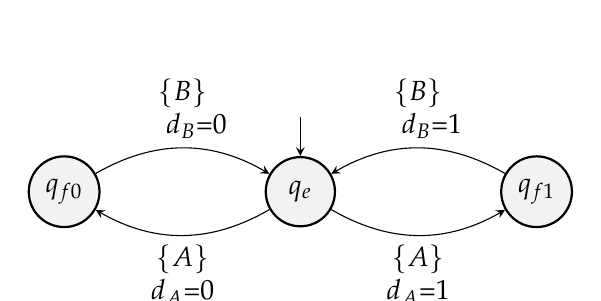
\begin{tikzpicture}
	\node[state, initial above] (q0) {$q_{e}$};
	\node[state, left of=q0] (q1) {$q_{f0}$};
	\node[state, right of=q0] (q2) {$q_{f1}$};
	\draw
	(q0) edge[bend left, below] node{$\{A\}$\\$d_A$=0} (q1)
	(q1) edge[bend left, above] node{$\{B\}$\\\hspace{1em}$d_B$=0} (q0)
	
	(q0) edge[bend right, below] node{$\{A\}$\\$d_A$=1} (q2)
	(q2) edge[bend right, above] node{$\{B\}$\\\hspace{1em}$d_B$=1} (q0)
	;
	\end{tikzpicture}
	\caption[CA for fifo1 connector.]{CA for the \textit{fifo1} protocol with ports $A$ and $B$ sharing data domain $\{0,1\}$.}
	\label{fig:fifo1_ca}
\end{figure}

Later, CA were extended to include \textit{memory cells} (or \textit{memory variables}) which act as value stores whose contents \textit{persist} into the future. Data constraints are provided the ability to assign to their \textit{next} value, typically using syntax from temporal logic (eg: $m'$ is the value of $m$ at the next time stamp). Figure~\ref{fig:fifo1_ca_mem} revisits the \textit{fifo1} protocol from before. With this extension, the task of persistently storing $A$'s value into the buffer can be relegated to $m$, simplifying the state space significantly. This change also makes it possible to represent connectors for arbitrary data domains, finite or otherwise.



\begin{figure}[ht]
	\centering
	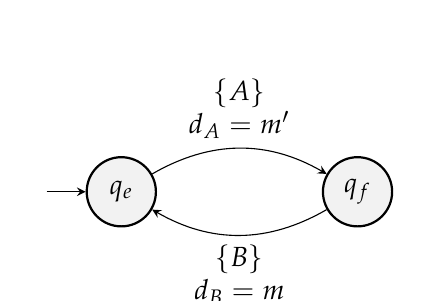
\begin{tikzpicture}
	\node[state, initial] (q0) {$q_{e}$};
	\node[state, right of=q0] (q1) {$q_{f}$};
	\draw
	(q0) edge[bend left, above] node{$\{A\}$\\$d_A=m'$} (q1)
	(q1) edge[bend left, below] node{$\{B\}$\\$d_B=m$} (q0)
	;
	\end{tikzpicture}
	\caption[CA with memory for fifo1 connector.]{CA with memory cell~$m$ for Reo connector~$fifo1$ with arbitrary data domain~$D$ common to ports~$A$ and~$B$. Two states are used to track to enforce alternation between filling and emptying~$m$.}
	\label{fig:fifo1_ca_mem}
\end{figure}


For the purposes of Reo, we are interested in being able to compute the composition of CAs to acquire a model for the compositions of their protocols. Figure~\ref{fig:fifo2_ca} shows an example of such a composition, producing \textit{fifo2} by composing \textit{fifo1} with itself. This new protocol indeed exhibits the desired behavior; the memory cells are able to store up to two elements at a time, and $B$ is guaranteed to consume values in the order that $A$ produced them. Even at this small scale, we see how the composition of such CA have a tendency to result in an \textit{explosion} if state- and transition-space. When seen at larger scales, a \textit{fifo$N$} buffer consists of $2^N$ states. The problem is the inability for a CA to perform any meaningful \textit{abstraction}; here, it manifests as the automaton having to express its transition system in undesired specificity. Intuitively, the contents of $m_0$ are irrelevant when $m_1$ is drained by $B$, but the CA requires two transitions to cover the possible cases in which this action is available. In the context of accepting existing trace tables, data constraints are evaluated predictably. However, in the case of code generation we are able to treat the data constraint instead as a pair of (a) the \textit{guard} which enables the transition as a function of the \textit{present} time stamp, and (b) the \textit{assignment}, which may reason about the next time step, and which we are able to guarantee by \textit{assigning} variables. As such, data constraints are broken up into these parts where possible. Figure~\ref{fig:fifo2_ca} and others to follow formulate their data constraints such that the guard and assignment parts are identifiable wherever it is practical to do so.


\begin{figure}[ht]
	\centering
	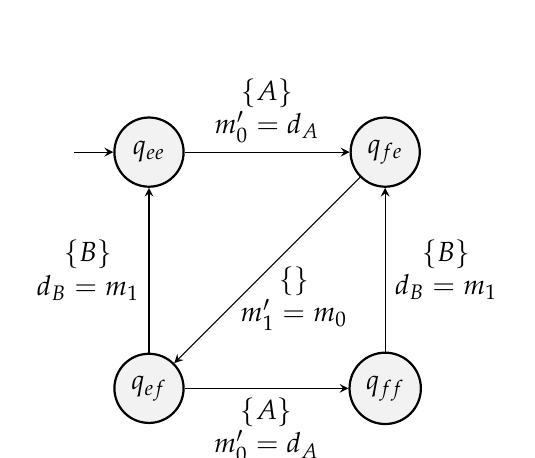
\begin{tikzpicture}
	\node[state, initial]      (qee) {$q_{ee}$};
	\node[state, right of=qee] (qfe) {$q_{fe}$};
	\node[state, below of=qfe] (qff) {$q_{ff}$};
	\node[state, below of=qee] (qef) {$q_{ef}$};
	\draw
	(qee) edge[above] node{$\{A\}$\\$m_0'=d_A$} (qfe)
	(qfe) edge[below] node[pos=0.43]{$\quad{}\{\}$\\$\quad{}m_1'=m_0$} (qef)
	(qff) edge[right] node{$\{B\}$\\$d_B=m_1$} (qfe)
	(qef) edge[below] node{$\{A\}$\\$m_0'=d_A$} (qff)
	(qef) edge[left] node{$\{B\}$\\$d_B=m_1$} (qee)
	;
	\end{tikzpicture}
	\caption[CA with memory for fifo2 connector.]{CA with memory cells $m_0$ and $m_1$ for the \textit{fifo2} connector with an arbitrary data domain for ports $A$ and $B$. Transitions are spread over the state space such that the automaton's structure results in the \textit{first-in-first-out} behavior of the memory cells in series.}
	\label{fig:fifo2_ca}
\end{figure}


\begin{figure}[ht]
	\centering
	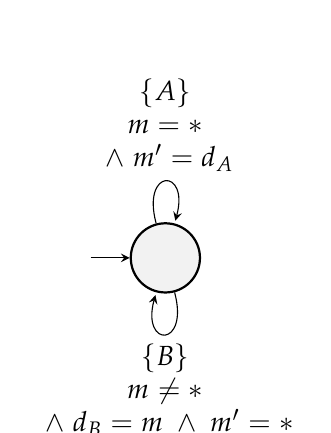
\begin{tikzpicture}
	\node[state, initial] (q0) {$ $};
	\draw
	(q0) edge[loop above] node{$\{A\}$\\$m=*$\\$\gapwedge{}m'=d_A$} (q0)
	(q0) edge[loop below] node{$\{B\}$\\$m\neq{}*$\\$\gapwedge{}d_B=m\gapwedge{}m'=*$} (q0)
	;
	\end{tikzpicture}
	\caption[RBA for fifo1 connector.]{RBA of the \textit{fifo1} connector for an arbitrary data domain common to ports $A$ and $B$. Memory cell $m$ is used both to buffer $A$'s value, and as part of the data constraint on both transitions for \textit{emptying} and \textit{filling} the cell to ensure these interactions are always interleaved. Data constraints are formulated for readability such that the `guard' and `assignment' conjuncts are line-separated.}
	\label{fig:fifo1_rba}
\end{figure}
Evidently, memory cells provide a new means of enforcing how data persists over time. In many cases, it can be seen that the same connectors can be represented differently by moving this responsibility between state- and data-domains. \textbf{Rule-based automata} (RBA) are the cases of CA for which this idea is taken to an extreme by relying only on memory cells entirely; RBAs have only one state. Figure~\ref{fig:fifo1_rba} models the \textit{fifo1} connector once again, this time as an RBA. Aside from the added expressivity, RBAs benefit from being cheaper to compose. As the state space is degenerate, RBAs may be easily re-interpreted into forms more easy to work with. \textbf{Rule-based form} (RBF) embraces the statelessness of an RBA as a single formula, the \textit{disjunction} of its constraints. In this view, Dokter et al.\ defines their composition of connectors such that, instead of exploding, the composed connector has transitions and memory cells that are the \textit{sum} of its constituent connectors\cite{dokter2018rule}.



\begin{figure}[ht]
	\centering
	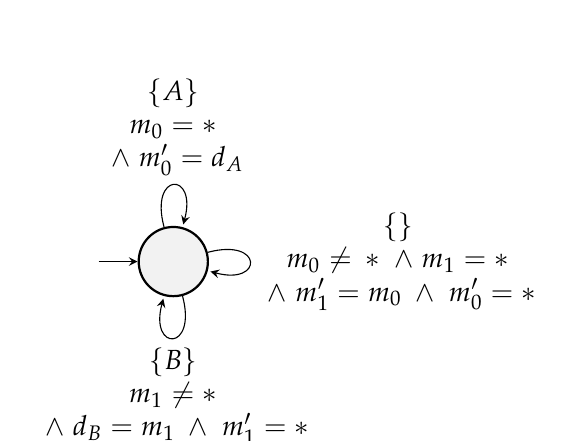
\begin{tikzpicture}
	\node[state, initial] (q0) {$ $};
	\draw
	(q0) edge[loop above] node{$\{A\}$\\$m_0=*$\\$\gapwedge{}m_0'=d_A$} (q0)
	(q0) edge[loop right] node{$\{\}$\\$m_0\neq{}*\gapwedge{}m_1=*$\\$\gapwedge{}m_1'=m_0\gapwedge{}m_0'=*$} (q0)
	(q0) edge[loop below] node{$\{B\}$\\$m_1\neq{}*$\\$\gapwedge{}d_B=m_1\gapwedge{}m_1'=*$} (q0)
	;
	\end{tikzpicture}
	\caption[RBA for fifo2 connector.]{RBA of the \textit{fifo2} connector for an arbitrary data domain common to ports $A$ and $B$. Memory cells $m_0$ and $m_1$ are drained by $B$ in the order they are filled by $A$, and have a capacity of 2 elements. Data constraints are formulated for readability such that the `guard' and `assignment' conjuncts are line-separated.}
	\label{fig:fifo2_rba}
\end{figure}



RBAs have a structure more conducive to \textit{simplification} of the transition space, such that one RBA transition may represent several transitions in a CA. Figure~\ref{fig:fifo2_rba} shows how how this occurs for the \textit{fifo2} connector. Where the CA in Figure~\ref{fig:fifo2_ca} must distinguish the cases where $A$ fills $m_0$ as two separate transitions, the RBA is able to use just one; likewise for the transitions representing cases where $B$ is able to drain $m_1$. This `coalescing' of transitions in RBAs is possible owing to the collapsing of their state space. Even without an intuitive understanding of why such transitions can be collapsed, such cases may often be identified only by inspecting the syntax of the data constraints. For another example of CA, a na{\"i}ve translation to RBA might produce two transitions with data constraints $m=*\wedge{}\;X$ and~$m\neq{}*\wedge{}\;X$ for some~$X$, which are both covered by a single data constraint $X$. As both RBA and RBF share this property, we usually refer to RBA transitions and RBF disjuncts as \textit{rules}, giving these models their name. By distinguishing CA transitions from RBA rules in terminology, we are perhaps more cognizant of the latter's increased ability to \textit{abstract} away needless data constraints. 

\begin{listing}[ht]
	\inputminted[]{java}{putget.java}
	\caption[Type state automaton in Java.]{An example of a program which implements a two-state automaton in the Java programming language. Observe that the behavior of states $A$ and $B$ are encoded implicitly in the \textit{structure} of the program, while determining which of the two in $A$ are available $A$ requires a check ar runtime.}
	\label{listing:putget}
\end{listing}
Typically, Reo has used the $Data$ domains in both CA and RBA as parallels to the data-types of the ports. In most of the languages in which Reo protocols are implemented, the discriminants of such types are not distinguished statically. For example, the C language lacks a way to statically enforce a that function \code{void foo(int x)} is only invoked when $x$ is prime. Instead, checks at runtime are used to specialize behavior. On the other hand, the state-space is simple enough to afford a practical translation into the structure of the program itself, requiring no checking at runtime. For example, Listing~\ref{listing:putget} shows an intuitive representation of a connector that alternates between states $A$ and $B$, getting data $x$ from its environment in $A$, and emitting $x$ when $x=3$. Observe that there is no need to protect operations behind a runtime-check of \textit{which} state the corresponding CA is in. This observation has implications for the behavior of implementations of RBAs, as they `cannot remember' which state they are in and must thus perform more checking. In practice, the overhead of this checking is manageable, and does not \textit{explode} under composition as the state space of CAs tend to do. The representation of automata in programming languages is explored in more detail in Section~\ref{sec:type_state}

\subsection{The Reo Compiler}
TODO ask Sung to summarize the history of the Reo compiler. give a summarized story here. 

The compiler aims to take the low-level implementation of a protocol out of the application developer's hands. Given a protocol specification, the compiler generates the \textit{glue code} and 

TODO focus on RBA

The steps from Reo specification to the generated glue code can be better understood when broken down into stages:

\begin{enumerate}
	\item \textbf{Specification expansion}\\
	The composed definitions of Reo components are unrolled to the channel-level until the protocol is represented by one large automaton with many nodes.
	
	\item \textbf{Minimization}\\
	Nodes not in the protocol's interface are \textit{hidden} and the RBA is minimized. This step produces a new, simpler automaton with the same behavior and interface.
	
	\item \textbf{TODO PUTTERS AND GETTERS}
	
	\item \textbf{Linking and Code Generation}\\
	The finished source code is generated from the resulting internal-representation. Those associated with functions in the target language are linked accordingly, and the rest are parsed and translated from the operational semantics of Reo to suitable target-language operations (such as data movement and duplication). The rules of the internal state are translated to the runtime definition of a protocol component object. An entrypoint to instantiating this protocol object is generated with the appropriate interface. The specifics of this step vary per target language.
\end{enumerate}

\section{Affine Types}

\cite{walker2005substructural}.
look for linear logic. proof theory. look into Rust's motivations. We can't pull things out of the blue. 

talk about TYPE-STATE pattern (aka state machine pattern)
https://hoverbear.org/2016/10/12/rust-state-machine-pattern/
http://cliffle.com/blog/rust-typestate/

\begin{verbatim}
pub struct X([u32;10]);
pub struct Y([u32;10]);


pub fn convert(x: X) -> Y {
Y(x.0)
}

pub fn do_thing_1(x: X) -> u32 {
x.0[0]
}
pub fn do_thing_2(x: X) -> u32 {
let y = convert(x);
y.0[0]
}
-------------------
example::convert:
mov     rax, rdi
mov     rcx, qword ptr [rsi + 32]
mov     qword ptr [rdi + 32], rcx
movups  xmm0, xmmword ptr [rsi]
movups  xmm1, xmmword ptr [rsi + 16]
movups  xmmword ptr [rdi + 16], xmm1
movups  xmmword ptr [rdi], xmm0
ret

example::do_thing_1:
mov     eax, dword ptr [rdi]
ret

example::do_thing_2:
mov     eax, dword ptr [rdi]
ret
\end{verbatim}

Type systems exist for the sole purpose of constraining which programs can be built, and do not add any expressiveness in terms of what can be computed. However, we know that adding (sensible) restrictions provides us other important properties. By constraining ourselves in some part, we drastically increase the number of properties that other parts are safe to assume. Affine types are a type system that applies this reasoning to explicitly managing access to variables, thus, allowing us to statically reason about resource management in a more fine-grained way. 

\subsection{The Rust Programming Language}
\label{sec:rust_language}
introduce Drop, Move, Clone, Copy

Aside from some unusual exceptions\footnote{TODO pinned objects}, all values in rust can be \textit{moved}, which describes a \textit{value} being transferred between variable bindings, or into functions as arguments, as demonstrated in Listing~\ref{listing:move}. Clearly, the Rust compiler tracks which values have been moved. Aside from preserving affine properties, this is necessary for determining when a value should be \textit{dropped}. \code{drop} is the \textit{destructor} function invoked by the compiler on a type when its binding goes out of scope and it has not been moved. 

TODO we use snippets from rust, but omit clutter such as visibility qualifiers, imports and sometimes variable names
TODo enum vs struct.
\begin{listing}[ht]
	\centering
	\inputminted[]{rust}{move.rs}
	\caption[Affine types in the Rust language.]{Type \code{Foo} is affine. On line 7, $x$ is moved into function \code{func}, consuming it. Accessing $x$ is invalid, and so line 8 raises an error.}
	\label{listing:move}
\end{listing}

\subsection{The Type-State Pattern}
\label{sec:type_state}

The \textit{state} or \textit{state machine} pattern refers to the practice of explicitly checking for or distinguishing transitions between and requirements of states in a stateful object\footnote{Usually, we disregard the effects of terminating the program. Equivalently, this pattern only allows one to describe automata in which every `useful' state reaches some final `terminated' state.}. Usually, these states are distinguished in the data domain of one or more types. Even the lowly \code{Option} type can be viewed as a small state machine as soon as some condition statement specializes operations performed with it.

The \textit{type state} pattern is closely related, but as the name suggests, it is characterized by encoding states as types, which usually are distinct from \textit{data} in their significance to a language's compiler or interpreter. A common approach is to instantiate one of the state types at a time. As an example, consider the scenario where a program wants to facilitate alternation between invoking some functions \code{one} and \code{two} which repeatedly mutate some integer $n$. Listing~\ref{listing:typestateeg} gives an example of what this might look like as a \textit{deterministic finite automaton} in the C language. In this rendering, the expression \code{two(one(START)).n} evaluates to the expected result of $(0 + 1) \cdot{} 2 = 2$. Even for this simple example, the encoding of states as types in particular has its benefits; the expression \code{one(two(START))} may appear sensible at first glance, but the compiler is quick to identify the type mismatch on the argument to \code{one}, making clear that the expression does not correspond to a path through the automaton:
\begin{verbatim}
note: expected 'DoTwo' but argument is of type 'DoOne'
\end{verbatim}

The type state pattern can be applied in any typed language, but it is particularly meaningful in languages where the compiler or interpreter \textit{enforces} its intended use. The example above demonstrates some utility, but a language such as C has no fundamental way to prevent the programmer from \textit{re-using} values. 
If the programmer misbehaves, they can retain their previous states when given new ones, and then invoke the transition operations as they please. It's not much of a state machine if all states coexist, is it? This is not always a problem in examples such as the previous. Here, the types prevent the construction of mal-formed \textit{expressions}, and perhaps this is enough. However, we cannot so easily protect a resource from any side effects of \code{one} or \code{two}; imagine the chaos that would result from these functions writing to a persistent file descriptor.
\begin{listing}[ht]
	\inputminted[linenos,tabsize=2,breaklines,frame=lines]{c}{typestate_eg.c}
	\caption[Type state automaton in C with expressions modeling runs.]{An example of the type-state pattern in the C language. The alternating invocation of \code{one} and \code{two} is translated to type-checking the compiler can guarantee. This example guarantees that well-formed \textit{expressions} can be interpreted as valid paths in some corresponding automaton, as the types must match.}
	\label{listing:typestateeg}
\end{listing}

An affine type system overcomes the shortcoming illustrated above. \hl{Formally, \textit{affine types} correspond with \textit{affine} substructural logic, in which the structural rule for `weakening' is absent; essentially, these logics do not consider terms to be idempotent.}
By treating instances of these types as affine \textit{resources}, the programmer cannot retain old states without violating the affinity of the types. The example looks very similar when translated to Rust, but now a case such as that shown in Listing~\ref{listing:typestateeg2} will result in the compiler preventing the retention of the variable of type \code{DoOne}.

\begin{listing}[ht]
	\inputminted[]{rust}{typestate_eg2.rs}
	\caption[Type state automaton in Rust with execution traces as runs.]{A demonstration of how the type-state encoding shown in Listing~\ref{listing:typestateeg} can leverage affine types to ensure that not only expressions, but \textit{a trace through execution} can be interpreted as valid paths through some corresponding automaton. The compiler correctly rejects this example, which corresponds with attempting to take transition \code{two} twice in a row.}
	\label{listing:typestateeg2}
\end{listing}

\subsection{Proof-of-Work Pattern}
\label{sec:proof_of_work}
Section~\ref{sec:type_state} demonstrates how the type-state pattern can be used as a tool to \textit{constrain} actions the compiler will permit the program to do. Indeed, this is a natural parallel to the affinity of the type system, which guarantees that no resource is consumed repeatedly. The counterpart to affine types is \textit{relevant} types, which defines correctness as each resource being consumed \textit{at least once}. Type systems that are both relevant and affine are \textit{linear}, such that all objects are consumed exactly once.

There is no way to create true relevance or linearity in user-space of an arbitrary affine type system; any program which preserves affinity is able to exit at any time without losing affinity. How are we able to enforce a behavior if it is correct to exit at any time? \textit{Proof-of-work} is a special case of the type-state pattern which allows the expression of a relevant type \textit{under the assumption that the program continues its normal flow}; ie. system exits are still permitted. The trick to enforcing the use of some object \code{T} is to specify that a type is a function which must \textit{return} some type \code{R}, and to ensure that \code{R} can \textit{only} be instantiated by consuming \code{T}. Clearly, we cannot prevent \code{T} from being destroyed in some other way, but we are able to prevent \code{R} from being \textit{created} any other way.

Realistic languages have many tools for constraining what users may access. Java has \textit{visibility} to prevent field manipulations. Rust has \textit{orphan rules} to prevent imported traits from being implemented for imported types. Languages without any such features won't be able to prevent users from creating the return type \code{R} without consuming \code{T}. In these cases, another option is \textit{generative types} which, among other things, allow us to further distinguish types with different origins. Here, generative types may be used to ensure not just \textit{any} \code{R} is returned, but a particular \code{R} within our control. As this work uses the Rust language for concrete implementations, we will rely on its ability to prohibit the user from creating \code{R} by using \textit{empty enum types} for types with no data nor type constraints, and by making its fields and constructors \textit{private} otherwise\cite{exotic_sizes}.

Consider the following illustrative scenario: We wish to yield control flow to a user-provided function. Within, the user is allowed to do whatever they wish, but we require them to invoke \code{fulfill}  exactly once (which corresponds to `consuming \code{R}'). How can we express this in terms the compiler will enforce? Listing~\ref{listing:promise} demonstrates a possible implementation (omitting all but the essence of `our' side of the implementation). The user's code would then be permitted to invoke \code{main} with their own choice of callback function pointer. Our means of control is the interplay between dictating both (a)
the \textit{signature} of the callback function and (b) prohibiting the user from constructing or replicating \code{Promise} or \code{Fulfill} objects in their own code.

\begin{listing}[ht]
	\inputminted[]{rust}{promise.rs}
	\caption[Proof of work pattern example of `promises'.]{A demonstration of proof-of-work pattern. Here, the user is able to execute \code{main} with any function as argument, but it must certainly invoke \code{fulfill} exactly once.}
	\label{listing:promise}
\end{listing}



\part{Contributions}
\chapter{Protocol Translation}
The Reo compiler has the task of translating a declarative protocol description to its target in some application language: Rust, in our case. In this chapter, we discuss how protocols are represented throughout this process, and how the transformation is achieved. 

\section{Two-Phase Translation}
The Reo compiler has an internal representation which corresponds closely to RBA, owing to the cheapness of \textit{composition}, as described in Section~\ref{sec:semantic_models}. As such, the majority of the work of the compiler's front-end is unrolling connectors, composing them into a large RBA. Existing back-ends perform the translation from this representation to the target languages directly. As a consequence, the Reo compiler itself contains a significant amount of \textit{language specific} details. For example, ports with unspecified types are represented with \textit{Object}, owing to this being a natural choice for Java. In this work, we introduce a new intermediate representation to ease the transition from the relational RBA form to the target language. As the name suggests, \textit{imperative form} aims to represent rules each as a sequence of imperative actions without including any specifics that tie it to any imperative language in particular. Next, we discuss the translation of this intermediate form to Rust in particular, and how the specifics of this process manifest. 
\hl{In previous works, reo generates the target code directly. }

\subsection{Motivation}
\begin{enumerate}
\item Removes work from the Reo back-end
\item 
\end{enumerate}
\hl{Reo's Java back-end generates t}

\subsection{Imperative Form}
\hl{In this work, we introduce a new intermediate representation for the reo compiler, which we will refer to as \textit{imperative form}. based on what can be described in an RBA. }

\subsubsection{Data Actions}
\hl{we implement synchronous interactions as a sequence of actions. this takes some care, as this translation gets hairy. eg: overwriting memory in the correct order. }

\subsubsection{Rules as Transactions}
\hl{
The Reo compiler has support for the TRANSFORM channel, which essentially allows the invocation of arbitrary functions in the circuit. eg $A=f(B)$ this gets complicated because these operations can be used in guards, assignments or both (as in $A=f(B)=m'$) the counter-intuitive thing is that the value must be computed to decide IF the rule may fire, yet we don't want the value if it does not. 
Instead, we model rule firings as TRANSACTIONS which can be rolled back. for every rule the last chance to roll back must precent the first VISIBLE EFFECT. 

we support this functionality with INSTRUCTIONS which are performed in sequence. these instructions can perform operations on data, such as creation of new elements, and it may trigger a ROLLBACK
}

\section{Code Generation}

\subsection{Reo Side}
\hl{we discuss the task of translating a declarative reo description into imperative form }

\subsubsection{Compiler Internal Representation}
\hl{compiler internal repr. is very similar to RBA with some extra information such as the direction of ports. some information is provided, such as figuring out the ASSIGNMENT to ports and memory cells}

\subsubsection{Group by Resource}
\hl{primarily want to find the mapping from putter to getters. this follows the FLOW of the DATA. ultimately we need}

\subsubsection{Type Constraining}
\hl{once the flow has been determined, we can see which operations must be supported on the target thing: mostly equality and clone operations. we wish to generate GENERIC protocols. so this requires TYPE CLUSTERNG and CONSTRAINING}

\subsection{Rust Side}
\hl{
imperative form is still too high-level to be used directly. what happens next is very language specific, and can be approached many ways. the section to follow explains how the final transformed rust works at runtime. Here, we concentrate only on getting it into that form.
}

\subsubsection{Runtime Interpreter}
\hl{many approaches are possible for translating the imperative form. in this work we go with an approach that is relatively abstract by implementing a lightweight INTERPRETER that is essentially instantiated with a small program that corresponds strongly with the abstract interpretive form. 
	This was done for several reasons: 
	1. extensive virtualization
	2. pushes protocol instantiation later into the instantiation process so more decisions can be made at the last moment
	3. represents more stuff as DATA relying less on monomorphization from generic types (as is the usual rust idiom), which makes it more inter-operable with C
	4. a data-oriented representation is more friendly to FFI. 
	5. runtime configuration}

\subsubsection{Checking and Errors}
\hl{Assuming that they are described using conventional data structures (sets, maps, lists, etc.) rba rules can be malformed. for example, checking a value not in the firiing set. As  Imperative form orients its description according to TIME and not VALUE, the operations on the same values are decoupled and spread out, creating many new possibiltiies of ill-formed operations. for example, moving a value that is only constructed later. These problems are familiar to sequential programming, as expected. the parallel is trying to manipulate a variable out of scope. etc.
To complement the throughline of "separating concerns", building a protocol object can FAIL, returning error. some failures are necessary for the build phase (eg: the builder does not know how to represent the movement of a value that has not been defined, as it does now know its data type), and other checks can result in sensible protocol objects but which would do something INVALID at runtime. for example, it would be possible to represent the consumption of a value whose name is in scope, but known to be EMPTY, but it would result in reading uninitialized memory at runtime.
}



\subsubsection{Optimization}
\hl{the INNER form of the rust protocol objects are indeed translated into a still more-complicated form for the purposes of optimization:
1. uses representations which are less convenient to use, but run more efficiently for their intended purpose (eg fusing port and memory readiness as they are usually checked togehter)
2. assumes that it is WELL FORMED to save the time that would be spent checking (eg: it can assume that a putter and getter expect the same data type. If it knows one, it does not need to look up the other)
}


\subsection{Function Calls}
\hl{Reo and RBAs in general support syntax for the TRANSFORM channel. these channels are particularly interesting because they blur the line between coordination and computation. in Reo, transform channels are intuitive: they output something which is a transformation of their input. done asynchronously, it is very clear to see how this would work. Unfortunately, Reo is synchronous which creates an interesting problem. Here, we see an instance of it in an RBA constraint: $f(P_0)=f(P_1)=C$. Let $P_0$ and $P_1$ be producers (they output into the protocol), and $C$ is a consumer, and $f$ is some unary function. This formulation has an interesting interpretation in the imperative realm: $C$ gets some datum that is computed using $f$, but \textit{only} if $f(P_0)=f(P_1)$. As $f$ is some arbitrary function, we must invoke $f$ before we know whether the result should be observed by $C$. }
\chapter{Protocol Runtime}
\label{sec:protocol_runtime}
Previously, Chapter~\ref{sec:imperative_form} described how a Reo protocol specification is translated by the Reo compiler into the Rust language as an executable protocol object. In this chapter we discuss how these objects are able to act as the \textit{communication medium} between a set of communicating omponents. This approach allows the user's component code to exchange data with its environment through the protocol object's exposed ports. Components make no assumptions about the world beyond their ports, and consequently, have no notion of the system in which they play a part. From a user's perspective, ports are entirely opaque, and their components may use them to exchange data with their environment without any concern for global coordination.

Internally, protocol objects orchestrate the actions on their boundary ports into interactions defined by its protocol specification. As much as possible, the protocol will work to facilitate data flow. However, whenever a boundary port initiates an action which does not yet fall into a suitable interaction, the protocol exercises its power to block its completion until the time is right. 

Section~\ref{sec:java_examined} begins by examining the Reo-generated protocol objects for the Java language, allowing us to use this previous work as a touchstone for our own. Within, Section~\ref{sec:java_observations} observes opportunities for our implementation to improve upon it by the addition of safety properties, and exploiting opportunities for optimization. Section~\ref{sec:requirements_defined} makes our goals explicit by defining the requirements and guidelines used to inform our design process and determine the assumptions used to facilitate out implemented optimizations.  Section~\ref{sec:protocol_objects} follows with the implementation of the \textbf{Reo-rs} library, which defines our protocol and port objects. Within, Section~\ref{sec:user_facing} explains how we leverage Rust's affine type system to expose a safe user-facing API. Sections~\ref{sec:chosen_design}--\ref{sec:behavior_implementation} explain how the protocol object behaves at runtime, detailing the implementation of optimizations which enable it to (1)~coordinate actions without needing a dedicated thread, (2)~increase parallelism by delegating data movement to component threads, and (3)~internally perform reference counting and reference passing while preserving Reo's semantics. Finally, Section~\ref{sec:requirements_evaluated} gives an overview of how our requirements and guidelines are satisfied, including references to the sections containing the relevant details.

\section{Examining the Java Implementation}
\label{sec:java_examined}
The Reo compiler has seen extensive development for its Java code generator in particular. In this section, we examine the properties of the source code it generates. Later, Section~\ref{sec:java_observations} makes particular note of opportunities for our own version to improve upon this design, or at least deviate to the end of specializing its implementation to better suit the Rust language.

\subsection{Architecture}
Fundamentally, the generated code adheres closely to Reo's literature, revolving around the interplay between \code{Port} and \code{Component} objects. From the perspective of a developer looking to integrate a generated Java protocol into their application, the entry point is the \code{Protocol} component (where `Protocol' is the name of the associated Reo connector).

Running a system requires an initialization procedure: (1) a \code{Port} is instantiated per logical port, (2) a \code{Component} is instantiated per logical component, and (3) pairs of components are linked by overwriting a port field for both objects with the same instance of \code{Port}. To get things going, each component must be provided a thread to enter it's main loop; in idiomatic Java, this manifests as calling \code{new Thread(C).start()} for each component \code{C}. A simplified example of the initialization procedure is shown in Listing~\ref{listing:java_gen_1} for the simple `sync' protocol which acts as a one-way channel. In this example, the ports are of type \code{String}.


\begin{listing}[ht]
	\centering
	\inputminted[]{java}{java_gen_1.java}
	\caption[Reo-generated Java protocol initialization.]{A simplified example of initialization for a system centered around a \code{Sync} protocol object, which acts as a channel for transmitting objects of type \code{String}. Both ports and components are constructed before they are `linked' in both directions: each port stores a reference to its components, and each component stores references to its ports. The system begins to run when each component is given a thread and started.}
	\label{listing:java_gen_1}
\end{listing}


In a sense, this implementation primarily hinges on \code{Port} as a communication primitive between threads, and equivalently, between components. For matters of concurrency, operations on port data involves entering a critical region. In contrast, \code{Components} are used only to store their ports and to be used as name spaces for their \code{run} function which implements their behavior (which corresponds to RBA rules in the case of the protocol component). Essentially, anything that interacts with \code{Port} objects can reify a logical component, whether or not this is done by an object implementing the \code{Component} interface.

\subsection{Behavior}
The representation of protocol rules is very intuitive; a rule is implemented as a block of code which operates on a component's ports. Once generated into Java, the only obvious sign that a component was generated from Reo is its linkage to multiple other components. The (simplified) generated \code{Component} code of the `sync' protocol from the previous section is shown in Listing~\ref{listing:java_gen_2}. This demonstrates that rules are indeed commandified, in that their behavior is encoded in discernible structures (appropriately called \code{Command}).

The behavior and structure of a component go together, and are generated by Reo at a relatively granular level. As such, the encoding of memory cells is natural also. Memory cells can be found next to ports in the fields of a \code{Component}.

\begin{listing}[h!]
	\centering
	\inputminted{java}{java_gen_2.java}
	\caption[Reo-generated Java protocol class of the sync connector.]{A simplified example of a Reo-generated Java protocol class for the $sync$ connector. By convention, it is started by invoking \code{start}, which is a method inherited from the \code{Runnable} interface which \code{Component} extends. This method assumes that all ports are correctly initialized and linked to another `compute' port. Its RBA-like behavior comes from an array of guards and commands which it iterates over in a loop, firing rules as possible forever.}
	\label{listing:java_gen_2}
\end{listing}

\subsection{Observations}
\label{sec:java_observations}
Reo-generated Java objects have a very clear correspondence to their declarative Reo specification. This carries over to how components and ports are used by an application developer. For example, Port objects act both as points of data exchange and as primitive concurrency mechanisms aligning \code{put} with \code{get}. From this design, we observe the following noteworthy properties:

\begin{enumerate}
	\item \textbf{Protocol Event Loop}\\
	Protocols are fundamentally passive in that they do not act until acted upon. Nevertheless, protocols each have their own dedicated thread that waits in a loop for a \textit{notification} from its monitor. Notifications originate from a component's own \code{Ports} in the event of a \code{put} or \code{get} invocation. For this reason, protocols and components are related in both directions, afforded by setting a port variable in one direction, and functions \code{setProducer} and \code{setConsumer} in the other.
	
	True to the intuition behind the RBA model, the protocol must check which (if any) commands can be fired, and keep spinning, trying rules while any guard is satisfied. This is unfortunate, as this approach requires guards to be evaluated repeatedly. As the protocol relies on the actions of other components to make progress, it is counterproductive for it to spend a lot of system resources evaluating guards to $false$. In cases where threads must share processor time, the excessive work of the protocol component will begin to get in the way of other components making progress, in turn leading yet more guards to evaluate to $false$.
	
	\item \textbf{Reference Passing}\\
	Java is a managed programming language whose garbage collector is central to how the language works. To support the transmission of arbitrary data types, \code{Port} is generic over a type. The language only supports this kind of polymorphism for objects. Unlike primitives (such as \code{int}), the data for objects is stored on the heap and is garbage collected by the Java Virtual Machine. Variables of such objects are therefore moved around the stack by reference. Moving and replicating values is cheap and easy, as they always have a small (pointer-sized) representation on the stack.
	
	A minor drawback is the need for indirection when performing operations that need to follow the reference. For example, comparing two \code{Integer} objects requires that the \code{int} primitives backing them on the heap be retrieved and compared. Equality is an example of an operation that the Reo protocol thread can be expected to perform frequently. The cost of this indirection depends on a myriad of factors, but is at its worst when it results in new, spread out locations each time. This case might arise, for example, if the \code{Sender} continuously created new \code{Integer} objects and sent them through its port. Another drawback is the requirement to allocate primitives on the heap before they can be sent through a port. This is not usually a problem in the case of Java, as in practice, almost everything is going to be stored on the heap with or without Reo.
	
	This aspect of the generated Java code will require the most change for the Rust version, as Rust has a very different model for memory management; it does not use a garbage collector by default, and structures are stored first and foremost on the stack as in the C~language.
	
	\item \textbf{Two Hops for Data}\\
	As protocols are components like any other, even the most trivial of data movements require values to hop at least twice: into the protocol, and out of the protocol. Fortunately, as stated above, the cost of the `hop' itself is trivial, as it will always be a small reference. The problem is the time delay between the hops, as it will often involve actions of three distinct threads in series (with the protocol in the middle). 
	
	\item \textbf{Vulnerable to User Error}\\
	The construction and linking of components with ports is not something the protocol itself is concerned with. Indeed, every component assumes that their port variables will be initialized by their environment. At the outermost level, this environment is in the application developer's hands. Components make no attempt to verify that they are correctly linked according to the specification; currently, there is not any infrastructure in place to support this checking if it were desired. As a result, it is possible make mistakes such as fusing two of a protocol's ports into one. Whether this is a problem worth solving depends on the burden of responsibility that Reo intends to place on the end user. These difficulties cannot be completely avoided, but approaches exist to minimize these opportunities for mistakes.
	
	While ports are clearly directional `from the inside out' (ports store distinct references to their producer and consumer components), the same is not so `from the outside in'. Neither of a port's components is prevented from indiscriminately calling \code{put} or \code{get}. The assignment of a port's values for `producer' and `consumer' component is in user space also. As a consequence, these fields may not agree with the components that interact with the ports at all. In fact, any number of components may store a reference to a port, each arbitrarily calling \code{put} and \code{get}. If done unintentionally, this would lead to lost wakeups; the thread blocking for a notification after calling acting on the port is not the same as the thread receiving the notification. Solutions can be conceived to wrap ports in objects that constrain the API of a port to one of the two `directions'. However, without affine types, there is no obvious way to ensure the number of components accessing a port is correct. In Rust, limiting these accesses becomes feasible.
	
	\item \textbf{Port Data Aliasing}\\
	In Reo, it is common for connectors to replicate port data. Owing to the nature of Java, this is currently achieved by duplicating references, where replication is also known as \textit{aliasing}. For immutable objects, aliasing has no observable side effects, and thus does not threaten Reo's value-passing semantics. However, Reo ports permit instantiation with any \code{Object}. Even if the operations are thread-safe, this causes incorrect behavior, as a component might observe their data changing seemingly under their feet. Worse still, objects which are not thread-safe can cause undefined behavior. This is a result of Java's view on memory safety having inverted priorities to Rust. In Java, operations are unsafe by default, and the programmer must go out of their way to protect themselves from data races, access of invalid memory and corruption. In Rust, the ownership system is based on the prohibition of mutably-aliased variables. Achieving replication in Rust will require some effort to convince the compiler of safety before a program will compile.
	
	\item \textbf{Non-Terminating Protocols}\\
	Currently, Reo-generated protocol objects loop forever unless they raise an exception and crash. For protocols that can perform actions with observable side effects in the absence of other components, this is perhaps a good idea. However, in the majority of realistic cases, protocols are indeed passive, and cannot do meaningful work as the only component. Reo semantics tend to reason about infinite behaviors. However, real programs often do end, and it is desirable that the program's exit is not held up by an endlessly-blocked protocol thread.
	
	\item \textbf{Protocol Components Cannot be Composed at Runtime}\\
	(TODO is this the place to explain this?)
	Ports allow data to move from the putter (or `producer') and getter (or `consumer') components as an atomic operation by delaying \code{put} or \code{get} operations until their counterpart is called also. This causes problems for the implementation of RBAs with rules whose guards are predicated by the data they move. How can a protocol decide if it should fire as a function of values it can only obtain \textit{by} firing? This ability to reason about the future is currently still a luxury limited to models such as TDS. The Java implementation gets around this problem by introducing asymmetry between `compute' and `protocol' components. Protocols are allowed to \textit{cheat}. The \code{Port} object has additional operations to inspect a value without consuming it: \code{peek} and \code{hasGet}. However, this asymmetry means that composing two Java protocol components (by linking them with ports) does not result in a component with their composed behavior. Solving this problem in earnest requires continuously-connected protocols to reason about their distributed state, which is a problem beyond the scope of this work. Reo's relationship with liveness properties is explored in Section~\ref{sec:api}.
	
	\item \textbf{Sequential Coordination}\\
	The Java implementation is structured such with ports being the critical region between components. As protocols have multiple ports, at first glance it may appear that coordination events could occur in parallel. However, no communication through protocol $P$ happens without the single thread in $P$'s \code{run} method. Indeed, \code{put} and \code{get} operations can be started in parallel by the boundary components, but $P$ can only complete it's half of these operations sequentially.
	
\end{enumerate}

\section{Requirements and Guidelines Defined}
\label{sec:requirements_defined}
Following the observations of Roe-generated Java objects in Section~\ref{sec:java_examined}, we identify and make explicit the design choices and goals that inform the design and implementation of our own protocol objects for the Rust language. 
First, we identify a number of functional requirements, representing the goals which can be assessed for satisfaction without ambiguity.


\begin{enumerate}
	\item[$\boldsymbol{R_{value}}$] Preserve Reo's value passing semantics. No user interaction should contradict these semantics. This precludes data races as a result of aliasing values which the user considers to be independent.
	
	\item[$\boldsymbol{R_{init}}$] Prevent the protocol from being initialized in an inconsistent state. Prevent port objects from being unitialized, unsafely accessed in parallel, or incorrectly connected to the protocol.
	
	\item[$\boldsymbol{R_{ffi}}$] Facilitate a foreign function interface with other systems languages C and C++. Ports and protocol objects should be accessible from those languages as well as Rust, such that they can be constructed, used and destroyed.
\end{enumerate}

Not all useful properties can be meaningfully quantified by strict requirements. We identify a set of guidelines intended to focus the design process, and to form a basis for the assumptions that make meaningful optimizations possible. By their nature, these guidelines cannot be clearly satisfied. Instead, the extent to which guidelines are satisfied is motivated by argumentation, and supported by experimental evaluation in Chapter~\ref{sec:benchmarking} where applicable.

\begin{enumerate}
	\item[$\boldsymbol{G_{data}}$] Allow the transmission of large data types without requiring the user to move them from the stack to the heap. Minimize the number of times data must be moved in memory such that data transmission remains performant for types with large representations.	
	
	\item[$\boldsymbol{G_{fast}}$] Minimize the overhead of control operations for the protocol object to route payloads and perform bookkeeping. In particular, minimize the cost of evaluating the rules before one is selected for firing.
	
	\item[$\boldsymbol{G_{end}}$] Facilitate the protocol object being destroyed and its resources freed. Facilitate a means of detecting termination which is correct and ergonomic.
\end{enumerate}


\section{Protocol Objects}
\label{sec:protocol_objects}
Here, we detail the structure and behavior that cause our Rust protocol object type, \code{Proto}, to coordinate the actions of boundary ports at runtime in accordance with its associated Reo specification. Section~\ref{sec:user_facing} details the user-facing API, and explaining how its helps to provide safety properties. Protocol objects offer an expansive design surface, and so Section~\ref{sec:chosen_design} relates our implementation at a conceptual level to that of the Java version that came before. Section~\ref{sec:protocol_object_architecture} lays out the structural definition of \code{Proto}, which is relevant for understanding its connection to the code generation process and imperative form explained in Chapter~\ref{sec:imperative_form}. Finally, Section~\ref{sec:behavior_implementation} details the implementation of \code{Proto}'s behavior at runtime, explaining the roles of the boundary components, how actions are arranged into interactions, and the effects of our implemented optimizations.

\subsection{Application User Interface}
\label{sec:user_facing}
The Reo compiler generates protocol descriptions in imperative form, which then are transformed by Reo-rs into runnable objects. The user therefore interacts mostly with Reo-rs itself, and Reo provides only the entry point for building particularly instances of protocol object. In this section we explain which functionality of Reo-rs is user-facing, focusing primarily on which requirements are satisfied.


\subsubsection{Construction and Destruction}
\label{sec:construction_and_destruction}
Reo-rs is built to interface with the Reo compiler, but it is not dependent on it. The entry point for protocol objects is the \code{ProtoDef} type, which is a concrete realization of the (logical) imperative form. For a concrete example, the previous chapter includes Listing~\ref{listing:generic_resolve}, exemplifying a \code{ProtoDef} representation of a simple imperative form. Regardless of whether the constructed \code{ProtoDef} was Reo-generated, it is instantiated along with any initial memory cells (in the \code{MemInitial} structure) to produce a \code{ProtoHandle}. This type has a small, pointer-sized shallow representation (i.e., 32 or 64 bits) to the \code{Proto} structure on the heap. The handle is opaque to the user, at first glance offering no functionality other than replication (safely aliasing the \code{Proto}) or destruction. If the the last handle to a \code{Proto} instance is destroyed, all of its resources are freed. This is achieved by relying on the canonical \code{Arc} type, (`atomic reference-counted') for the definition of \code{ProtoHandle}.

The protocol remains inert until the user acquires some of its ports. However, they cannot be constructed independently. Instead, the user must invoke \code{claim} on a \code{ProtoHandle}, which identifies the port through the inclusion of a parameter specifying the port's logical name; this corresponds with the symbolic name as it appears in the imperative form. By encoding both its orientation (i.e.,\ \code{Putter} or \code{Getter}) and its data type as type parameters for each port object, \code{claim} is able to reflect on these properties and return an error (Section~\ref{sec:rust_language} explains how Rust represents exceptions with enumeration types) if the port's properties are incongruous with the protocol's definition, or if the port of that name is currently claimed. Similarly, port objects notify their \code{ProtoHandle} that their name is again available to be claimed in the event of their destruction. All together, this API is able to guarantee that (1) every logical port has at most one port object at once, and that (2) the types of ports enforce that their orientation and data type align with their specification.

\code{Proto} objects are stored on the heap, but their ownership is shared between all of their existing \code{ProtoHandle}s. Internally, ports contain a \code{ProtoHandle} each also. These handles are thin wrappers around Rust's \code{Arc} (`atomic reference-counted') type, ensuring that the handles are moved, acted upon and destroyed in a thread-safe manner. Once the last handle is destroyed, the \code{Proto} is destroyed also, freeing all of its resources in the process without a trace. \code{Proto} objects do not rely on any static variables, allowing any number of them to be instantiated and used throughout a program without them interfering with one another's execution (except, of course, their sharing of the underlying hardware resources). 

\subsubsection{Port Operations and Variants}
\label{sec:port_operations}
The API that defines \code{put} and \code{get} operations for ports is partitioned over port types in the expected way. Concretely, ports are represented in Reo-rs by distinct types \code{Putter<T>} and \code{Getter<T>}, each generic over their data type, where \code{get} is only defined for getters, and \code{put} is only defined for putters. In both cases, the operations rely on Rust's borrowing rules to ensure that even if the port objects is shared within the user's program, it is impossible to act on a port from two threads concurrently (without circumventing the Rust compiler with \code{unsafe} operations. For example, the signature of \code{get} is specifies that the getter is accessed via a mutable reference\footnote{This terminology is often confusing; despite the name, `mutability' is more often used to mean `mutually exclusive', as is the case here. The Rust compiler will only permit this operation in a context where it is certain that the port is not concurrently being used elsewhere.} (written~\code{\&mut}).

The \code{get} operation blocks the calling thread until an element of type \code{T} is returned. Users are able to customize their involvement in the interaction by invoking one of \code{get}'s variants. For example, \code{get\_timeout} blocks the thread up to a specified timeout, and returns an \code{Option<T>} to distinguish success from failure. The latter case represents the failure to participate in an interaction, allowing the caller to reclaim the control flow and continue working. Getters also have the option of calling \code{get\_signal}, which expresses a wish to participate in an interaction, but no desire to acquire the datum. The utility of this option is that Reo-rs will attempt to avoid the work of acquiring the value at all, potentially avoiding a \code{clone} operation and other associated overhead (explained in Section~\ref{sec:data_exchange}). The effects of this variant on performance are shown in Section~\ref{sec:benchmarking}. \code{get\_signal\_timeout} is also available, and behaves as expected.

Similarly, putters have access to \code{put\_timeout}, which varies from~\code{put} in the expected way. Both operations have the potential to return the putter's value. This may occur even if the value was involved in an interaction, but was not acquired by any getters. Returning the value allows the user's program to decide what to do with the value. For example, a user may decide to put the value again until it is read. If this behavior is undesired, putters offer the \code{put\_lossy} and \code{put\_timeout\_lossy} variants which will not return the value regardless of the actions of getters, dropping it if needs be.

\subsubsection{Value-Passing API Semantics}



The Rust language conflates the movement of values to new variable bindings with two meanings: (1) the value's ownership is transferred to the new binding and scope, and (2) the value's shallowest representation is moved in memory. Reo's semantics require that the data transmitted through ports is truly \textit{moved}, transferring ownership. Clearly, not doing so would violate Reo's semantics; values acquired through ports might be dropped or acted upon at the whims of their original putter, of which the getter would have no knowledge. As is idiomatic for the Rust language, our API transfers ownership into the scope of \code{put} and out of the scope of \code{get} by moving the value itself. Na\"ively, this has significant performance implications, as the cost to move a value is dependent on the size of its representation. For example, a 10MB array is significantly more costly to move than a byte. For cases where the relocation of bytes is not necessary, Rust programmers can often rely on LLVM to optimize the memory movements away, passing consumed resources by reference `under the hood' (but retaining the semantic movement of ownership). However, these optimizations are not guaranteed. Users of the Rust language have grappled with this shortcoming for years, but the search for a satisfying solution remains an open problem~\cite{matsakis_2015}. The only way to guarantee that the data is passed by reference at runtime is to expose an \code{unsafe} API, which relies on the user to pass references and manage the associated ownership manually. Our requirements prioritizing safety ($\boldsymbol{R_{value}}$) and performance ($\boldsymbol{G_{data}}$) are in conflict. Our solution is to compromise by exposing these options to the user as variants for \code{put} and \code{get}, and allow them to decide on a case-by-case basis: 

\begin{enumerate}
	\item \textbf{Value passing.}\\
	We expose safe functions \code{put} and \code{get} to consume and return data by value, guaranteeing correctness. Depending on the compilation environment, it may require up to two moves of the data.
	
	\item \textbf{Reference passing. User provides correctness.}\\
	Operations are parameterized by references (or raw C-like pointer types) which Reo-rs writes to and reads from directly. The caller takes responsibility for ensuring that the value at the pointer's destination is initialized or dropped as necessary to correspond with Rust's usual ownership system. For example, this version of \code{put} is given a pointer to initialize memory, which the operation will initialize.
	
	\item \textbf{Value pass a `referring' type.}\\
	As far as Reo-rs is concerned, this is indistinguishable from case~(1). However, the user intentionally reinterprets the data types of their ports such that they represent indirections. For example, \code{Box<T>} is a pointer-sized owned type which will be transmitted by Reo-rs much like any other pointer-sized integer, oblivious to the fact that it indirectly represents another type \code{Q}. Taken to the extreme, a na\"ive solution replaces all data types with heap-allocated indirections, inheriting the associated downsides shared with the Java implementation. Other approaches may be simple (eg: transmitting an index to a shared vector) or arbitrarily complicated (Several Rust libraries exist for decoupling an object's data from its ownership, such as \code{rent\_to\_own}, \code{managed} and \code{swapper})\footnote{These libraries are publicly available on \url{crates.io}.}. 
\end{enumerate}

To reflect our priority of safely, the `default' port operations use value passing, corresponding to options (1) and (3). Users are able to take safety into their own hands by opting into \texttt{*}\code{\_raw} port operation variants. We rely on Rust's idiom of marking such operations as \code{unsafe}, communicating to the user that they are adopting the responsibility of reading the API documentation to determine and provide the necessary guarantees, as is usual in languages such as~C; this keyword requires the user's code to be explicitly qualified as an \code{unsafe} block, making it impossible for them to easily overlook this requirement. 

\subsubsection{Interface with C and C++}
Programming languages rely on an \textit{ABI} (application binary interface) for translating functions and types into binary according to a dependable convention. When languages agree on this interface, it ensures that both caller and callee with agree on the minutia of the calling convention, and how structures are laid out in memory. It is common for Rust, C and C++ to interface using the C ABI, and as such, there is syntactic support for selecting the ABI to be used per function and per structure. Reo-rs makes use of this feature to expose C-friendly types and functionality as part of its foreign function interface. In most cases, this requires nothing more than the addition of preprocessor annotations, i.e.,\ \code{\#[repr(C)]} and~\code{\#[no\_mangle]}, and visibility keywords, i.e.,~\code{extern}.

Rust makes frequent use of generic type parameters, which rely on the Rust compiler for dispatch at the call site (see Section~\ref{sec:rust_language}). C has no analog for this feature, and thus, some structures and functions are be provided secondary concrete representations. As an example, Rust represents the \code{Putter} and \code{Getter} types with a generic argument, affixing its data-type at compile-time. Reo-rs preserves safety guarantees by relying more extensively on reflection at runtime for these cases.

Rust has no analog to C's header files; it does have trait-associated functions, which can declare functions without defining them. However, they are of no use here, as they are not usable from C, as they are inherently coupled with Rust's generic system. To facilitate the sort of workflow that is idiomatic to C, whereby definitions and declarations can be distinguished such that \textit{compilation} can be distinguished from \textit{linkage}, the Rust ecosystem offers an addon for generating C header files from Rust source. This module can be loaded as the \texttt{bindgen}\footnote{url: \url{https://crates.io/crates/bindgen}.} addon to Cargo, Rust's package manager (comparable to Pip for Python, NPM for Node-js, and perhaps Maven for Java). With this tool, we are able to generate C~header files without much friction, and include them in any distributions such that downstream dependents on Reo-rs can incorporate them into their applications as they would do for any other C library. Once compiled and linked, their~C or~C++ applications would execute as would any other binary, and the use of Rust for compiling Reo-rs is no longer visible. Owing to its nature, calls that cross the Rust-C boundary do not induce any significant overhead~\cite{klabnik2018rust}.

\subsection{Design Process}
\label{sec:chosen_design}
Many designs for the implementation of Reo-like coordinators are possible. Their structure and workings all depend on how information is arranged, and how multiple threads come together to coordinate on an a priori unknown task without stepping on one another's toes. In our case, we concentrate on the case where all participants in the system share a memory address space, which opens up many means of exchanging data between threads.\footnote{This assumption provides context for our work, but is not an inherent assumption of all of our design choices. Wherever possible, we make this distinction in the text.} As is typical in multithreading, the problem is not accessing the data, but rather restraining oneself from accessing the data at the wrong time. Before we can approach any design decisions, we examine what we know for certain: ports invoke \code{put} or \code{get}, each from their own thread. They cannot return immediately, as this would not result in the correct system behavior; when not aligned in time, getters will often (unknowingly) read uninitialized data, and putters will write their data, never to be read. They wish to exchange data in accordance with some defined protocol, but a priori have no knowledge of the protocol, nor their role in it. The aim is to facilitate rule firing `greedily' as opportunity allows: i.e.,\ protocol objects should fire rules as frequently as possible such that the behavior of the system is not constrained \textit{beyond} the constraints of the protocol itself.

\subsubsection{The Coordinator}
The most obvious starting point is asking `who decides which rule to fire?' Reaching consensus prevents the system from reaching some malformed state where two rules are being committed to in tandem, violating the protocol or deadlocking on some resource they have in common. It is easy to contrive of such examples where numerous ports are involved. For example, consider a case where two rules disagree on which of two putter ports distribute their datum to a set of getters. If not done carefully, some getters may receive one value, and the rest another. The most approachable solution is to stick more closely to the Reo model by introducing a specialized \textit{coordinator} for each protocol. Consensus is trivial when one participant is elected the leader for every circumstance. Unfortunately, we cannot rely on some port $x$ being involved in every rule firing such that they are the coordinator. Many protocols do not have such an $x$ that can be relied upon to be present. The Java back-end solves this problem by adding a fresh `protocol' thread whose task is to only coordinate the others. This approach is easy to think about, as there is a clear mapping from threads to roles. However, the protocol thread is not inherently coupled to the actions of ports. It has to wait for opportunities to coordinate, necessitating the transmission of explicit events from compute threads to the coordinator. These messages can use a channel, or use something like semaphores or monitors to send signals instead, and then relying on the coordinator to rediscover which ports are ready by reading the state of shared memory. Next, one must decide who organizes the actions into an interaction. The Java backend's approach is to spread ports out over space such that they can become ready concurrently.\footnote{Conceptually this could be in parallel, but the actual implementation the exchange necessitates the use of a \textit{class monitor lock} (a structure for coordinating actions for all instances of a class) to prevent interfering with the protocol thread itself.} The coordinator then treats the port structures like messaging pigeonholes, and performs the task of moving data around itself. The coordinator's notification to the ports is subtle; taking the form of \code{put} and \code{get} calls which release port-local locks, unblocking the compute threads, completing the interaction. This solution is effective, but has some downsides, as discussed in Section~\ref{sec:java_observations}. 

\subsubsection{Event Handling}
A minor change with the potential for improvement is to remove the necessity of the protocol thread to rediscover the nature of the event which generated a wakeup signal. Rather than signals with no payload, we can use events which carry explicit information, eg: `Port $x$ is ready to get!'. With this approach, the coordinator waits in an event loop, handling incoming events. The Rust ecosystem has a number of libraries for defining event loops built atop system signal handles. An early implementation made use of the \code{mio} crate for sending events which communicated \textit{which} port has become ready. With this minor change, the coordinator does not need to inspect the contents of ports directly, which, owing to their modification by multiple threads, inherently cause several cache misses for the coordinator. Rather, the coordinator is able to manage a private, dense, redundant record of which ports are ready. Aside from the unfortunate data duplication, this optimization contributes greatly to the satisfaction of $\boldsymbol{G_{fast}}$. Unfortunately, regardless of how fast \code{mio} may be, the event must still cross the boundary between threads. In overburdened systems, this has the consequence of causing context switches.

\subsubsection{Threadless Protocol}
If the coordinator has its own `protocol thread', threads focus on their own work; the coordinator coordinates, and port threads interact with their ports. However, for all interactions that involve one or more ports (which are frequent in practice) we observe that despite the presence of multiple specialized threads, their tasks are not concurrent. Port threads perform external work until they instigate a port operation, until the coordinator is woken up to complete the interaction by firing the rule. Port threads and coordinator cannot know when to act, and must rely on notifications from one another. Threads must wake up and go to sleep frequently. 

One pivotal decision of our final design is to attempt to alleviate this problem. If compute threads are going to block, waiting for progress anyway, why not have them do the coordination themselves? In our approach, we discard the dedicated protocol thread and reinterpret the coordinator as a \textit{role} which the other threads take turns adopting. Conceptually, this change is a minor one; there is ultimately still at most one thread acting as coordinator. Until now, we have taken for granted that the coordinator can complete interactions with impunity; as they are the only elected leader of their kind, there is no concern for data races. In our new model, if anyone can be a coordinator, we must go our of our way to prevent two threads from adopting the role at once. Where before the bottleneck existed (implicitly) as a single coordinator thread processing a sequence of events one at a time, we now make the lock explicit: upon becoming ready, every thread attempts to acquire the \textit{protocol lock}, the holder of which acts is the only coordinator for the duration.

\subsubsection{Delegating the Task of Data Exchange}
Owing to our focus on values at the systems level, we do not have the simplifying luxury of the Java backend to presume that moving data is cheap. In Rust, as in C and C++, values are not represented by indirect references by default; often, their shallowest representations are all there is to them. To satisfy $\boldsymbol{G_{data}}$, the Java backend's (admittedly intuitive) representation of ports as data pigeonholes is wasteful. For many realistic Reo protocols, data often moves through protocols synchronously, moving from \code{Putter} to \code{Getter} without any storage in memory cells in between. 

Our implementation introduces a new idea in an attempt to capitalize on this observation: getters fetch their data directly from the source. In this approach, the coordinator does not necessarily handle data itself. Rather, it decides which rule to fire and delegates the task of moving the data to the getters themselves. In addition to skipping a redundant `data hop' from putter to coordinator, this also facilitates the dissemination of a putter's datum to all its getters in parallel. This change requires extra messaging form the coordinator, as getters are given more responsibility. Where before a signal from coordinator to getter sufficed (`Your datum is ready!'), coordinators must now communicate the location of the getters' source (`Your datum can be found at~$P$!'). Note that this idea is applicable in a context where components are distributed, i.e.,\ they do not all share an address space. In such cases, it becomes vitally important to manage the task of data movement for the sake of performance, which is likely to complicate this optimization further. 


\subsection{Architecture}
\label{sec:protocol_object_architecture}
\code{Proto} is a type corresponding closely to its imperative form specification type, \code{ProtoDef}. While they represent the same thing, their differences in structure and contents are a result of them being used for different purposes. Despite the increase in granularity from Reo's RBA-like form, \code{ProtoDef} still represents a specification of the protocol; as such, it strives to minimize redundancy to simplify parsing and minimize the surface for internal inconsistency. On the other hand, \code{Proto} is structured to facilitate execution at runtime.

\begin{enumerate}
	\item \textbf{Layout optimized for speed.}\\
	As discussed in Section~\ref{sec:translation_phase_2}, the \code{build} method is the only user-accessible means of constructing \code{Proto} instances. The methods of this type can rely on this to assume that their contents are internally consistent, thereby avoiding the cost of performing many checks at runtime. For example, if a rule's guard includes an equality check between the values in memory cells $m_0$ and $m_1$, \code{Proto} is able to assume that these cells have the same type; it is safe to use the result of $m_0$'s definition of type-equality.
	
	Additionally, concise structures can be rearranged such that their layout facilitates less computation time. A general example of this paradigm is caching. Here, a clear example is the replacement with symbolic names for ports, functions and memory cells (represented by strings in the \code{ProtoDef} type), using integers for keying into vectors, maps and other such structures directly.
	
	\item \textbf{Additional data for primitive concurrency.}\\
	Where \code{ProtoDef} can leave information implicit, \code{Proto} must be explicit. Interface ports require some data structures for storing concurrency primitives. For example, coordinators must send control messages to getters, as explained in Section~\ref{sec:chosen_design} above. 
\end{enumerate}

\subsubsection{Critical Region}
Section~\ref{sec:chosen_design} explains how threads initiating actions at boundary ports of a protocol assume the role of coordinator. It is fruitful to examine the fields of \code{Proto} in accordance to which roles access them, and how their access is safely controlled. The most coarse-grained distinction is that between fields inside and outside the protocol's lock-protected critical region. This divide is so fundamental, that is is immediately apparent by looking at the definition of \code{Proto} itself, seen in Listing~\ref{listing:proto}. \code{ProtoCr} stores all of the fields manipulated only by the coordinator, such as the \textit{allocator}, to which the coordinator delegates the task of storing persistent values. This is explained further in Section~\ref{sec:memory_cells} to follow. Also observe the field responsible for managing which ports are \textit{claimed} (See Section~\ref{sec:port_operations}). While this is not a task traditionally associated with the coordinator, it's mutually exclusive access between threads necessitates that this structure is protected by the lock.

\subsubsection{Spaces}
Clearly, \code{ProtoCr} can contain only the data that is not contended by multiple threads. Some structure is still needed for threads to rendezvous such that information can be exchanged and actions can be aligned in time. In the Java implementation, the class \code{Port} served two distinct purposes: (1) stored the value being exchanged by two threads, and (2) acted as the rendezvous for putter and getter. As explained in Section~\ref{sec:chosen_design} above, the former of these tasks does not involve the coordinator in Reo-rs. However, the latter is still relevant. To meet this need, \code{ProtoR} associates a \code{Space} for every identifier (for ports and memory cells alike). The difference is name exists to distinguish them from ports, to which they are certainly related, but not identical. For every identifier, its \code{Space} contains precisely the data needed for it to communicate with its peers. For ports, this includes a \code{MsgBox}, which serves as a control-message channel from coordinator to compute-thread. Spaces are discussed further in Section~\ref{sec:data_exchange} to follow. 

\begin{listing}[ht]
	\centering
	\inputminted{rust}{proto.rs}
	\caption[Proto type with parts inside and outside the lock.]{Definitions of the most coarse-grained structures of a protocol instance. \code{Proto} is the entrypoint, composed of \code{ProtoCr} in the critical section, accessed by only the coordinator, and \code{ProtoR} outside it, accessed by all.}
	\label{listing:proto}
\end{listing}


\subsection{Behavior}
\label{sec:behavior_implementation}
This section explains how the data structures of the \code{Proto} type comes to life at runtime to emerge as coordination according to the protocol with which it was configured. 

\subsubsection{Rule Interpreter}
Unlike the Java implementation, Reo-rs moves the specification of the protocol type very late into the pipeline from Reo to the final application. Rather than relying on Reo to generate native application code, in this work we make more extensive use of the virtualization pattern. At runtime, the coordinator traverses rules in data form, performing tasks as a rudimentary \textit{interpreter}. The tasks associated with such a \code{Rule} correspond closely to the conceptual interpretation of the imperative form. At this granulairty, interactions do not exist explicitly. Rather, the interpreter must perform the work associated with each rule interaction as a sequence of actions which, all together, appear to the observer as an interaction. For simple rules, it is clear to see how such interactions can be created. For example, consider a simple rule with constraint $P=C$ where $P$ and $C$ are putter and getter ports respectively. Here, $P$'s value is simply moved to $C$ if both ports are ready. As RBF rules become more complex, more actions become necessary to achieve the results of the interaction. Section~\ref{sec:imperative_form_sec} explains how by imperative form's restrictive representation already captures the result of this action-centric breakdown such that the interpreter does not need to compute it at runtime. These actions preserve their interaction-based semantics by behaving as \textit{transactions}, with actions clearly divided into two sequences around an instant where the rule can be thought to \textit{commit}. As long as their effects can be reversed, action prior to the commit can create temporary variables and trigger commit as they please. This approach is flexible enough to represent Reo's \textit{transform} channels, allowing values to be created and destroyed synchronously by being represented inside the transaction itself. 


\subsubsection{Minimizing the Bottleneck}
\label{sec:minimizing_the_bottleneck}
Reo-rs shares its centralized locking architecture with the Java backend. Regardless of whether the coordinator and the thread that performs the role are decoupled, the importance of providing it mutual exclusion is clear; two coordinators in tandem would not be safe in the knowledge that the state does not change between evaluating the guards and changing the state. Methods exist for fragmenting protocols such that the locking becomes finer grained as protocols are into sets of smaller ones. As such, the Reo compiler internally produces a set of protocols as its output, though the work on this feature is ongoing. Nevertheless, we consider this decomposition an orthogonal concern and consider it no farther. Reo-rs embraces this central lock, but takes measures to minimize the duration for which it is held. In this section we discuss these measures and how they work together to help satisfy $\boldsymbol{G_{fast}}$. To structure our reasoning, we identify the tasks a coordinator performs from the moment to acquires the lock (accepting its role), to the moment it releases it (relinquishing the role). 

\begin{enumerate}
	\item \textbf{Initialization}\\
	Section~\ref{sec:port_operations} explains how the time spent purely on overhead is diminished by avoiding the event-signal interaction used by the Java implementation, necessary to wake a sleeping protocol thread. Once the coordinator has acquired its lock (a task needed in both versions), transitioning into the work of the coordinator is nothing more than the time taken to invoke the \code{coordinate} function call.
	
	\item \textbf{Checking Readiness and Memory State}\\
	Imperative form shares the explicit representation of the synchronization constraint with RBAs, encoding precisely which ports are involved with the firing. Clearly, a rule cannot fire until all ports involved are \textit{ready}. Per port, this is a boolean property which can be represented by a single bit flag. Owing to the simplicity of this data, each of these sets can be represented as a single \textit{bit-vector}, a data structure for which set operations are exceptionally fast. Reo-rs takes this optimization a step further by extracting another boolean property per memory cell: fullness. The idiomatic encoding for memory cells storing data of type \code{T} in Rust would be the \code{Option<T>} type, such that \code{Option::None} represents emptiness. Instead, the relevant flags for fullness are extracted, separated from their data and instead coalesced into another bit-vector. With just a handful of fast bit-wise operations, the coordinator is able to quickly detect whether a rule cannot fire, as a result of a port not being ready, or a memory cell being full when it should be empty, or empty when it should be full. In practice, the vast majority of cases where a rule's guard is unsatisfied are detected in this step.
	
	
	\item \textbf{Instructions}\\
	Instructions are relatively expensive compared to the other steps in a rule's interpretation. Their cost scales with their complexity, as they can be defined as arbitrarily large and deep formula terms. Even individually, the cost of each operation can be high, as they include arbitrary user-defined function invocations, arbitrary user-defined equality checks, and allocation space for newly-created data objects. Section~\ref{sec:memory_cells} explains how the cost of memory allocation is mitigated such that the allocation itself is amortized to constant time. For the rest of these operations, there is not much that can be done to avoid the cost; for the most part, they would be expensive even if each rule were performed by a native Rust function. Fortunately, the vast majority of rules for Reo connectors require no instructions at all. In practice, Reo connectors tend not to inspect the data whose flow they coordinate. The more intrusive the protocol's routing logic becomes, the more it begins to resemble computation (i.e.,\ not coordination), a task for which Reo should probably not be optimized. For the protocols without instructions (including $fifo1$, $alternator$, $sequencer$, $sync$, and more), the support for instruction parsing costs no more than the time to determine that there are zero instructions to execute.
	
	\item \textbf{Movements}\\
	Once a rule is committed, the role of the coordinator is to kick any getters into action, delegating the data exchange to them. Each movement encodes one resource (\code{Putter} or memory cell) being distributed amongst a set of \textit{recipients} (each a \code{Getter} or memory cell). This meta interaction is not synchronous; getters may take arbitrary time before waking up and actually participating in the data exchange. This is not the case for memory cells; as part of the configuration of the protocol, this is manipulated by the coordinator only. As such, operations which move values \textit{into} memory (where memory cells act as getters) are performed first. Section~\ref{sec:memory_cells} explains this procedure in more detail. Here, it suffices to say that the movement of memory between memory cells is fast.
	
	For port-getters, the coordinator does not move the value itself. Rather, the work is delegated to the compute-thread by sending a control message to the getter's \code{MsgBox}. 
	
	Usually, the coordinator does not have to interact with the resource (acting as putter) at all. It can rely on getters to `clean up'. The coordinator returns, releasing the protocol lock. The only exception is for movements with zero getters. Such cases can represent a resource being destroyed. In these cases, there is no getter to perform the cleanup, and so, the coordinator does it itself. For a \code{Putter}, this is no more than sending a control message, releasing it. For memory cells, this may require running the \code{drop} function associated with the memory cell's data type.  Section~\ref{sec:memory_cells} provides more detail on how these are managed.
	
\end{enumerate}

\subsubsection{Data Exchange}
\label{sec:data_exchange}

Eventually, each \code{Getter} waiting at their \code{MsgBox} receives a control message from the coordinator, revealing to them the identifier from which they must fetch their value. Their task is to locate the corresponding \code{Space} and contend with an unknown number of fellow getters to complete the movement. The correctness of this exchange relies on the satisfaction of a number of properties:
\begin{enumerate}
	\item \textbf{One getter cleans up the resource}\\
	Regardless of whether the resource is a \code{Putter} or a memory cell, the set of getters are responsible for cleaning up the resource to finish the interaction. In the case of a putter, this takes the form of sending them a control message, notifying them that everyone has finished inspecting their datum and they may return to the caller. Clearly it is unsafe for anyone to release the putter before some getter has finished reading the datum; by returning, the putter may invalidate the memory region storing the datum.
	
	In the case of a memory cell resource, cleanup takes the form of resetting its ready-flag inside \code{ProtoCr}, signifying that the memory cell is in a stable state can again be involved in rule firings. This is necessary as there is no dedicated thread guaranteed to set this flag in future, as is the case for getters and putters. Section~\ref{sec:memory_cells} to follow also explains how these memory cells are emptied in these events such that they can again store new values. This manipulates the protocol's state, potentially making new rules' guards satisfiable. As such, this last getter must once again acquire the protocol lock and attempt to \code{coordinate}.
	
	\item \textbf{At least $N-1$ getters \code{clone}}\\
	Rust generalizes the operation for replicating a datum to produce another instance from it. It is idiomatic to rely on the standard trait \code{Clone} with single operation \code{clone} to implement this behavior. This approach covers cases for which there is a non-trivial means of replicating objects; sometimes, performing a bit-wise copy of the structure's shallowest representation is not enough. Consider the example of \code{Arc} (`atomic reference-counted') in Rust's standard library. This type consists of just a pointer to some heap-allocated tuple \code{(refcount, data)}, and is used for shared, reference-counted ownership of \code{data}. For this type, coping the pointer to the tuple is not sufficient. Cloning must follow the pointer and increment \code{refcount}.
	
	\item \textbf{One getter moves instead of cloning}\\
	Data movements represent the transmission of data from source to a set of destinations. Generally, the value is no longer present at the source afterwards. Na\"ively, the original must be dropped to complete the interaction. However, it is wasteful and illogical to replicate an object only to destroy the original. Instead, we wish to move a value between threads, much as Rust's move semantics allow the movement of affine types between bindings. This cannot be done in the conventional way, as movement is defined is generally within the context of a single thread and scope. Regardless of Rust's expressiveness, it is nonetheless an action-centric language, and does not offer the interaction we need.\footnote{Rust is able to understand uni-directional movement of values into new threads using the same mechanism by which closures can enclose variables in their parent scope. More complex types are able to also create their own notions of safe `movement' by composing actions as we suggest in this section. As in our case, they require the use of \code{unsafe}, as by definition the Rust compiler cannot reason about their correctness in the usual way.} 
	
	When orchestrated correctly, we are able to implement a safe move operation between threads by invoking a pair of \code{unsafe} operations, one on either end. In unsafe Rust it is possible to copy a value without influencing the original. If not done correctly, this can easily lead to double frees. On the other hand, it is possible to leak resource memory with \code{forget}, an operation of Rust's standard library which causes the compiler to consider the value moved without invoking \code{drop}. These pitfalls should be familiar to C programmers, as unsafe Rust gives one the capability to interact with `raw' pointers in a fashion similar to that of~C. Together, these actions constitute the inter-thread move primitive we need.
	
	We elaborate our task by requiring an election between getters, such that one is designated the \textit{mover}, and the rest are \textit{cloners}. 
	
	\item \textbf{All clones must be complete before the move}\\
	It is unsafe to move a value before or while performing \code{clone} on the original. Essentially, every data exchange must proceed in two strict phases such that all clones occur in the first, and the move in the second.
	Consider again the example of type \code{Arc} by examining this sequence of events that results in undefined behavior: (1) \code{Arc} $x$ represented by a pointer to heap region at $p$ is moved to binding $y$. (2) $y$ goes out of scope, it's \code{refcount} is reduced to zero, and so its heap allocation is freed. (3) \code{Arc::clone} is invoked with $x$, which traverses its pointer to memory position $p$, and attempts to increment \code{refcount}. $p$ is no longer allocated, and arbitrary memory corruption ensues. To prevent such cases, Reo-rs must take care to order all clones of some value before it can be moved, as the Rust compiler would do.
\end{enumerate}

Many solutions are possible, but have in common that these getters must exchange some meta-information safely across thread boundaries. Our solution uses a pair of atomic variables for this purpose, \textit{count} and \textit{mover}, initialized by the coordinator a priori to $N$ and $true$ respectively. In a nutshell, mover is true if no getter has yet claimed the role of mover, which represents both (1) the responsibility to clean up, and (2) the privilege of moving the original value, rather than cloning it. Part of the procedure at large is a pair of elections between getters to determine a mover and a \textit{last} getter. We elect a mover first. The time between the elections gives the losers (the `cloners') the opportunity to clone, safe in the knowledge that the mover will not clean up until they are finished. If the mover is also elected last, they clean up and return immediately, as all clones must already be complete. Otherwise, the mover must await a signal from whomever is last before cleaning up.

This process is complete enough to implement the desired functionality for \mbox{Reo-rs}. However, we identify two important optimization opportunities which have the unfortunate consequence of complicating the data exchange procedure further.
\begin{enumerate}
	\item \textbf{Not all getters want data}\\
	Getters participating as a result of the \code{get\_signal} operation will not return a value. Clearly these getters cannot avoid participating in the mover election, as then nobody would clean up. These getters specialize their interactions by participating in the last election first. The intuition is that if they lose this election, it is safe for them to return without participating in the mover election; clearly this covers the case of no getters wanting the data. It is also safe to rearrange these elections in this case; these getters have no intention to \code{clone}, and thus are not a threat to the invariant that required these elections to be ordered in the first place: all clones are complete by the time the last getter is
	
	\item \textbf{\code{Copy}-types can be replicated without \code{clone}}\\
	Section~\ref{sec:rust_language} explains how \code{Copy} marks types for which have a trivial destructor, and are safe for multiple getters to replicate by copying their value bit-wise. This is the case for primitives, and structures composed entirely out of primitives, such as arrays of integers. 
	
	For copy-types, the mover and the copiers may copy the original datum in parallel. Afterward, only the last getter is elected to clean up, safe in the knowledge that all copies are finished.
\end{enumerate}

The full data exchange procedure is spelled out in Rust-like pseudocode in Listing~\ref{sec:data_exchange} in the Appendix.

\subsubsection{Memory Cells}
\label{sec:memory_cells}
Section~\ref{sec:protocol_object_architecture} explains that per \textit{location} (generalizing ports and memory cells), Reo-rs maintains a persistent \code{Space} structure at a fixed location on the heap such that threads have a predetermined location to rendezvous on communication primitives. Section~\ref{sec:data_exchange} follows up, explaining how these structures are also pivotal to data exchange. When getters converge on the space of a \code{Putter}, they rely on the presence of a prepared data reference in the space to the location of the putter's datum on its own stack. In this manner, values moving between ports are never moved to the heap at all. The memory alignment of the putters datum generally differs per data exchange, necessitating that their space's reference be updated to the location of their value each time. 

Memory cells differ from putters in that their value \textit{persists} beyond the lifetime of any individual thread participating in the protocol; consequently, the data itself \textit{must} be stored on the heap. A na\"ive implementation treats memory cells similarly to putters by continuously \textit{updating} the data reference in the associated \code{Space} such that it points to a freshly allocated value on the heap every time the memory cell is filled.

We are able to rely on a property of Reo for an optimization: memory cells have predefined types. Instead of shifting the pointer around to a fresh allocation each time, we are able to \textit{preallocate} the space needed to store one value per memory cell. In this model, the references do not change. Instead, each has a single allocation which is repeatedly reused. Whenever the cell is empty, the contents of the allocated space are \textit{uninitialized}. This can be done safely by relying on auxiliary structures for tracking when memory cells are empty; Section~\ref{sec:minimizing_the_bottleneck} explains how \textit{bit vectors} serve this purpose for Reo-rs. This approach removes the cost of creating and allocating spaces at runtime. Unfortunately, this approach suffers a drawback inherited from its strict interpretation of \textit{value-passing semantics}: moving data between memory cells is expensive. While small optimizations are possible for some circumstances (e.g.,\ we are able to swap references when the contents of two memory cells are \textit{swapped}), they are only applicable in a handful of situations. 

Requirements~$\boldsymbol{G_{data}}$ and~$\boldsymbol{G_{fast}}$ incentivize a more extensive optimization. Reo-rs intentionally decouples memory cells (including their spaces and their fullness flags) from \textit{storage}, which describes where the contents of the cells is kept on the heap. We observe that Reo protocols perform logical replication of values often, while mutating existing values rarely. As such, many situations exist in which we are able to safely \textit{alias} values between memory cells by relying on \textit{reference counting}. We extend the idea of reusing allocations, but rather that fixing them per memory cell, we allow all memory cells of the same data type to draw from a shared pool of reused allocations; this is often referred to as an \textit{arena allocator}. The intricacies of this process are delegated by the coordinator to the \code{Allocator}, which tracks which \textit{storage cells} of a type are available (free) and which are occupied. Rules which replicate, destroy or move data between memory cells thus can often moving data altogether, instead manipulating only the references within spaces, and reference counters of storage cells. For example, a rule which empties memory cell $m_0$ (destroying the contents) needs to only decrement the reference counter. Only when the counter reaches zero does the allocator need to be involved, invoking the value's \code{drop} function in place and freeing the storage slot. This approach has another advantage: \code{clone} is invoked \textit{lazily}, in some cases being avoided altogether. Consider a connector for which values originate from putters, get stored in memory slots, are replicated repeatedly, only to be destroyed before ever being emitted to a getter. In this example, \code{clone} is never necessary. This approach has an additional consequence; the data exchange operation explained in Section~\ref{sec:data_exchange} may be initialized such that \textit{nobody} is permitted to move. The procedure already given (in Listing~\ref{sec:data_exchange}) is able to handle this case.

\subsubsection{Type Reflection}
\label{sec:type_reflection}

Section~\ref{sec:rust_language} explains how Rust offers both static and dynamic dispatch for executing generic code, similar to how it is done for C++. These options offer a trade-off in runtime speed, binary size and flexibility. Reo-rs cannot hope to rely on static dispatch to resolve the concrete types of port data, as they are only discovered later in the moment our \code{Rule} structures are interpreted. The idiomatic approach to such situations is to rely on dynamic dispatch, which virtualizes the operations on some generic type by adding indirection which is resolved at runtime through the traversal of function pointers. As with C++, Rust uses \textit{virtual function tables} (`vtable') for this purpose. Dynamic objects are stored in place with a pointer with the relevant vtable, and operations traverse the table according to a statically-defined layout to resolve the concrete functions. Clearly, this is only possible if the method creating the dynamic object and the operations on it agree on the vtable's contents. To this end, Rust relies on its trait system: dynamic objects are created and interacted with in terms of some trait, which provides it with both an interface and a type. As such, Reo-rs defines a trait \code{PortDatum}, which defines all the operations belonging to all port data: (1) how is the object laid out in memory, (2) how are objects checked for equality, (3) how are objects cloned, etc. Two problems present themselves with this idiomatic approach:
\begin{enumerate}
	\item Who defines \code{PortDatum} for the user's data types? The idiomatic approach is to expose the trait and simply require the user to implement the trait's associated operations to their type. However, if we do not trust the user entirely, some of our desired optimizations become impossible.\footnote{This is a limitation of Rust's trait system, which prohibits the inclusion of associated functions and properties for traits used for the creation of dynamic objects. Rust does not support representing them in the vtable. This limitation may be removed in future.} For example, users must mark their objects as \code{Copy}, communicating that their shallow representation can be safely copied in memory. 
	
	\item How do we express types of \code{PortDatum} which do not implement an equality or clone operator? These may not be defined for the type. One is able to express Reo connectors which will not use these operations (and thus is is correct not to require them), but we cannot know whether they are used statically.
\end{enumerate}

We solve both of these problems by using an experimental feature the Rust language not yet available in the stable version: \textit{specialization}. With this feature, we solve the first problem by defining \code{PortDatum} for every conceivable generic type ourselves, with their fields populated as a function of the type's properties. In this manner, \code{PortDatum} can be made entirely private, benefiting the user in alleviating their need to implement it, and benefiting Reo-rs by guaranteeing it is implemented correctly for every type. This also solves the second problem; as \code{PortDatum} is under our control, we can provide dummy implementations for operations which the type does not define, such that all \code{PortDatum}-implementor types can use the same vtable layout, despite differing in the subset of the trait's operations they define. Conceptually, we can represent undefined functions with null pointers in the vtable. For safety's sake, we instead use dummy functions which trigger an explicit panic, unwinding the stack and throwing unrecoverable errors in the event a programming oversight attempts to traverse these undefined function pointers. Listing~\ref{listing:specialization} gives a simplified\footnote{The real trait definition contains more fields, and must perform some manipulations of raw pointers to get around Rust's restrictions on which traits may be used for dynamic dispatch. For this reason, it is important for us to control its definition for any type~\code{T}. These details are omitted for brevity.} view of the \code{PortDatum} trait, and its implementation for any\footnote{In the final implementation, we must include some trait bounds for all \code{PortDatum} types. \code{Send} and \code{Sync} are common Rust marker traits for types that can be passed between threads by value and reference respectively. They are implemented by default for all reasonable types such that users almost never need to consider them~\cite{klabnik2018rust} (they are derived for user-defined types by default also), but this requirement covers some prickly safety pitfalls.} data type,~\code{T}.

\begin{listing}[ht]
	\centering
	\inputminted{rust}{specialization.rs}
	\caption[Rust specialization to implement traits.]{Using Rust's specialization feature to define \code{PortDatum} (simplified) for every generic type~\code{T} by relying on \code{T} always implementing helper traits \code{MaybeCopy} and \code{MaybeClone}. \code{MaybeCopy} can be implemented for any~\code{T}, defining a default behavior in one block, and then overriding it for a more specialized behavior in the other. The Rust compiler will resolve which block to use based on the static properties of \code{T}, deriving a \code{PortDatum} implementation with precisely the desired definition. In this manner, \code{PortDatum} can be made inaccessible to the user, allowing Reo-rs to trust that it was defined in the expected manner. The helper traits are necessary to satisfy the requirements of the specialization feature: there must be a strict ordering on the specificity of implementation blocks for the same trait.}
	\label{listing:specialization}
\end{listing}

Rust's chosen representation of dynamic objects is the \textit{fat pointer}, which represents a dynamic object as a pair of pointers, one to its \textit{data} (i.e., some structure with fields), and one to its \textit{behavior} (i.e., the vtable). These trait objects can be thought to carry their behavior around with them; they move with their vtables. While ergonomic in general, this is often redundant in the case of Reo, where values are guaranteed to only move between ports and memory cells of the same type anyway. In our case, we would repeatedly overwrite these tuples to overwrite the \textit{data}, and redundantly overwrite the vtable pointer with an identical one. This is a symptom of Rust's approach to dynamic objects in general; it `resolves' their concrete type \textit{per operation}. This approach is detrimental to Reo-rs for two reasons:
\begin{enumerate}
	\item Dynamic objects are accessible through their trait interface. Behind this interface, their concrete types are erased. There is no means to check type-equality between two dynamic \code{PortDatum} objects, as is needed during the \code{build} procedure (see Section~\ref{sec:translation_phase_2}) to ensure that memory is initialized with the expected type and so on.
	
	\item Dynamic objects carry their vtable pointers with them. This increases the size of their representation significantly (in the case of small types)
\end{enumerate}

Our solution is to implement our own dispatch system that makes use of Rust's native vtables and dynamic dispatch, but without the above properties. Essentially, we split Rust's fat pointers into their \textit{data} and \textit{behavior} components, using the former as data as usual, and using the latter as a \textit{key} to reflect on the concrete type's behavior as needed. Section~\ref{sec:imperative_form_sec} introduced the \code{TypeInfo} type, which appears to the user as nothing more than some \textit{identifier} for its type. Under the hood, this value is the vtable pointer itself, thereby usable as a \textit{key} to identify the type and to reflect on the behavior of some dynamic~\code{PortDatum} object inside Reo-rs. Listing~\ref{listing:reflection} shows how function \code{TypeInfo::of} provides the user with the only means of creating a \code{TypeInfo} for some~\code{T}. Only in the creation of the \textit{imperative form} structure (the \code{ProtoDef} type) does Reo-rs accept the user's provided \code{TypeInfo} directly, as it would be unsafe to rely on the user providing some \code{T} with a matching \code{TypeInfo}. Instead, the API of Reo-rs includes one layer of \textit{static dispatch} into the library where necessary such that the creation of the \code{TypeInfo} can be trusted. For example, when populating some \code{MemInitial} structure with the initial values of memory cells (as described in Section~\ref{sec:translation_phase_1}), values can only be input with the \code{with} function. The user uses Rust's safe dispatch system, oblivious to Reo-rs translating their concrete objects into dynamic ones behind the scenes. For example, the user might see:~\code{MemInit::default()::with("hello")}, and Reo-rs would resolve the \code{TypeInfo} for \code{\&'static str} type behind the scenes.


\begin{listing}[ht]
	\centering
	\inputminted{rust}{reflection.rs}
	\caption[Tricking Rust into exposing a vtable.]{`Tricking' the Rust compiler into retrieving the vtable of a given type \code{T} for dynamic dispatch to virtual functions of trait \code{PortDatum}. The safe cast on line~7 inserts a pointer to a vtable which the compiler will ensure is present in the program text. \code{TypeInfo} structures can later be used for type reflection, by manually appending this pointer to reconstruct the fat pointers that Rust natively uses for dynamic dispatch.}
	\label{listing:reflection}
\end{listing}

Listings~\ref{listing:refl_test_in} and~\ref{listing:refl_test_out} in the appendix demonstrate how \code{TypeInfo::of} appears in the generated binary.

\section{Requirements and Guidelines Evaluated}
\label{sec:requirements_evaluated}
In this section, we give a summary of the means by which the requirements and guidelines of Section~\ref{sec:requirements_defined} are satisfied and adhered to respectively. This doubles as an overview of this chapter at large, motivating its points by referring to the relevant subsections above.


\begin{enumerate}
	\item[$\boldsymbol{R_{value}}$] Values passing through ports preserve value-passing. This is achieved even in the presence of reference-passing optimizations `under the table' by leaning on the same philosophy that Rust uses to prevent data races: prohibit mutable aliasing. Objects are only aliased (accessible via multiple bindings) if they are be identical. Section~\ref{sec:port_operations} explains how protocols limit aliasing to their internals by relying on value-passing port operations. On the other hand, Reo-rs aliases values, but only until they are mutated. Section~\ref{sec:memory_cells} explains how memory values are safely aliased.
	
	Section~\ref{sec:imperative_form_sec} explains how Reo-rs interprets an imperative form protocol description at runtime, relying on a transaction-like model to safely allow the creation of new values to be incorporated in synchronous interactions. In this manner, protocols whose rules create and reason about temporary values can be faithfully represented.
	
	\item[$\boldsymbol{R_{init}}$] Section~\ref{sec:user_facing} explains how users are shielded from the granular initialization procedure by exposing an API with explicit constructor functions \code{build} and \code{claim} of protocols and ports respectively. Protocol objects are extensively customizable by the expressiveness of imperative form, with which \code{build} is parameterized. At the same time, these structures are kept internally-consistent by the preservation of invariants, and relying on \code{build} as the only user-facing means of instantiation.
	
	\item[$\boldsymbol{R_{ffi}}$] C and C++ foreign-function interfaces are provided by relying simply declarations with the C ABI where possible. As C cannot support Rust's notion of generics, where necessary, the \code{ffi} module provides generic-free alternatives for data types and functions where generics are represented as data instead. Reo-rs can thus be compiled once into either a statically- or dynamically-linked library for use in these other languages without any additional runtime overhead.
	
	\item[$\boldsymbol{G_{data}}$] Reo-rs facilitates the transmission of any fixed-size data types by value. This permits but does require data to be heap-allocated. Sections~\ref{sec:data_exchange} and~\ref{sec:memory_cells} explains how Reo-rs has a value-passing API, but relies on reference-passing to minimize the number of times values are moved in memory.
	
	\item[$\boldsymbol{G_{fast}}$] Section~\ref{sec:chosen_design} explains Reo-rs coordinates the actions of multiple threads while minimizing the overhead of inter-thread communications. Section~\ref{sec:minimizing_the_bottleneck} explains how meta-operations are represented such that they can be batched, allowing the coordinator to reduce the overhead of processing rules for firing.
	
	\item[$\boldsymbol{G_{end}}$] Section~\ref{sec:chosen_design} explains how protocol objects are not given their own threads, trivially facilitating termination detection if no ports remain to interact with it. Section~\ref{sec:construction_and_destruction} describes how protocol structures are implicitly cleaned up once all of their ports are destroyed. 
\end{enumerate}
\chapter{Generating Static Governors}
\label{sec:api}

The cumulation of the previous chapters describe a stand-alone contribution to the Reo compiler. We have seen that users are able to generate Rust source code from a Reo specification (Chapter~\ref{sec:imperative_form}) which may be used in conjunction with their own Rust code to behave according to the corresponding protocol specification at runtime (Chapter~\ref{sec:protocol_runtime}). The programmer is able to rely on these protocol objects to constrain the behavior of their program at runtime such that no deviations from the protocol specification may be observed. 

In this chapter, we design the \textbf{governor generator}, a tool to augment the user's Reo-coordinated Rust programs. As with the Reo compiler before, this tool generates a Rust source file from the Reo protocol specification which the user may import as a dependency. Within, a Rust type which corresponds with a \textit{governor}. If integrated into the implementation of the user's components, the Rust compiler will enforce that the user's code does not \textit{inhibit} the behavior of the system at large. In effect, users are provided an ergonomic means to opt-into their Rust compiler enforcing \textit{liveness} properties of their programs. 

Section~\ref{sec:governor_defined} provides the formal definition of \textit{governors}, and how they relate to protocols, components and liveness. Section~\ref{sec:unintended_constraints} describes the problem the \textbf{governor generator} aims to solve from the perspective of a Rust programmer relying on Reo to coordinate their components' communication. Section~\ref{sec:soluition_static_governance} gives a high-level overview of our corresponding solution. Section~\ref{sec:making_it_functional} explains in detail how the \textbf{governor generator} works, concentrating only on what is required to make it minimally-functional. Finally, Section~\ref{sec:making_it_practical} elaborates on the means by which the solution is made ergonomic and practical.

\section{Governor Defined}
\label{sec:governor_defined}
A Reo protocol specification defines which interactions are permitted between its boundary ports. In other words, protocols \textit{constrain} the behavior of any system of which they are a component. This is the result of Reo's semantics, which 
guarantees that the behavior of a system is the composition of its components at any granularity. However, protocols do not prevent their boundary components from adding constraints of their own. As a consequence, the definition of a component viewed in isolation does provide any guarantees on which interactions \textit{are} observable in the system at large. To make this possible, a component needs some knowledge about the behavior of the system beyond its own ports. Fortunately, Reo specifications take us halfway there, as they make explicit which behaviors they permit in an unambiguous form that can be transformed and inspected. To proceed, we define the \textit{governor}.

Protocol $P$ with interface ports $I_P$ defines $G_{P,I_P}$, its governor with respect to its interface ports. $G_{P,I_P}$ shares interface $I_P$ with $P$ itself, and also constrains the interactions between them in the same manner as~$P$. However, all port actions in $G_{P,I_P}$ are the \textit{complement} of those in $P$, ie.\ all \textit{puts} are \textit{gets} and all \textit{gets} are \textit{puts}. $G_{P,I_P}$ characterizes the behavior of a component that, if connected to $P$ with interface $I_P$, would result in a composite system with the same behaviors of $P$ itself. In other words, $G_{P,I_P}$ describes the behavior which $P$ would permit to occur, from the perspective of a component interfacing with \textit{all} of $P$'s ports.

Governors are generalized such that they are defined for any \textit{subset} of a protocol's interface ports, ie.\ a protocol $P$ with interface $I_P$ defines a set of governors $\{G_{P,x} \; | \; x\subseteq I_P\}$. Governors characterize the reverse-oriented behaviors as before, but such that these behaviors are \textit{projected} onto the governor's own interface; \textit{projection} is defined precisely by Baier et al.\ ~\cite{baier2006modeling}, and is explained in Section~\ref{sec:rba_projection} when it is needed. Here, it suffices to say that the behavior as constrained by the governor omits the actions of all ports not in the governor's interface. This captures the intuition that the governor only specifies the interactions of its own boundary ports, not constraining the actions of other ports at all. As such, the behavior of a governor is \textit{at most} as constrained as that of the protocol itself; for every port not included the interface, the governor potentially becomes more \textit{lenient}. This is made clear for the trivial case of a governor with the empty interface, which has no constraints whatsoever.

The utility of this construction is that it provides a means by which a component interfacing with some protocol $P$ with any of its ports may compute \textit{precisely} which behavior the protocol permits. By relying on the fact that protocol objects will facilitate any and all permitted interactions as possible at runtime, this boundary component is able to predict \textit{precisely} the behavior the component that arises from its composition with the protocol. In the simplest case, one is able to enforce that the resulting behavior matches the constraints of the protocol; equivalently, the protocol's boundary components do not contribute any behavioral constraints that the protocol itself did not define already. For such systems, one may understand the entirety of the system's coordination behavior by inspecting the definition of the protocol alone. In these cases, we say that the component is \textit{adherent} to the protocol.

\section{The Problem: Unintended Constraints}
\label{sec:unintended_constraints}
A central tenet of Reo's design is the \textit{separation of concerns}, part of which is the desire to minimize the knowledge a compute component must have of its protocol. In this view, coordinating the movements of data is not a concern relevant to the task of computation. A desirable balance is possible with the observation that protocol objects are able to partially impose protocol adherence on their neighbors; External ports may instigate a \code{put} or \code{get} at any moment, and the protocol will complete them as soon as the protocol definition allows it. In this way, coordinators possess a crucial subset of the features of \textit{governers}: aligning the \textit{timing} of two actions that compose an interaction. Unfortunately, in the properties of the realm of sequential, action-centric programming itself \textit{implicitly} imposes constraints on the behavior of the system: \code{put} or \code{get} block until their interaction is completed, and no subsequent code (potentially, other port operations) will occur until they do. This is beyond the capabilities of the coordinator to influence.

In the context of application development, this has an interesting consequence; the behavior of the system is influenced by the behavior of (potentially) all of its components. This is sensible in theory, but becomes unwieldy in practice. Even small changes to the behavior of a compute component influences the system's behavior in unexpected ways, as we are not used to thinking about synchronous code as a composable protocol, nor are we able to intuit the \textit{outcome} of the composition. For example, Listing~\ref{listing:transform_not} gives the definition of a compute function which a user may write to interact with a protocol. When \code{p} and \code{g} are connected to a \textit{fifo1} protocol (which forwards \code{p} to \code{g}, buffering it asynchronously in-between), it runs forever and the output will be something like:
\begin{verb}
	I saw true. I saw false. I saw true. I saw false. (...)
\end{verb}.\\However, when connected with the \textit{sync} protocol (which forwards \code{p} to \code{g} synchronously), the system has no behavior. The problem is that even though \textit{fifo1} and \textit{sync} have the same \textit{interface}, \code{transform\_not} is \textit{adherent} to the former protocol, but not the latter. By definition, \textit{sync} fires when both \code{p} and \code{g} are ready, but \code{transform\_rot} does not \code{put} until the \code{get} is completed. Once the intricacies of these programs grow beyond a programmer's ability to keep track of these relationships, the composed system may have \textit{unintended} behavior. This property may be obvious at the small scale of this example, but it becomes more difficult the larger and more complex the program becomes. In the worst cases, an innocuous change adds a new constraint such that no next interaction exists, manifesting at runtime as \textit{deadlock}. 


\begin{listing}[ht]
	\inputminted[]{rust}{transform_not.rs}
	\caption[Rust example of a compute component.]{A function in Rust which can be used as a compute component in a system, connected to a protocol component.}
	\label{listing:transform_not}
\end{listing}


%That said, the Reo compiler aims to generate code which describes \textit{eac}
%
%In this section
%
%1. intro to the problem at high level.
%2. you are writing a more complicated component. multiple ports yeah!
%3. oh no its not behaving as expected!
%4. section guide

%\section{Governors Defined}
%\label{sec:governor}
%In this work, we accept that it is necessary to write compute code that has blocking behavior. Rather than attempting to empower the coordinator with the ability to further influence its boundary components, we introduce explicit governors into our applications such that from the protocol's perspective, the components appear to manage themselves. A particular compute component requires a particular governor as the behavior permitted to the compute component is a function of its \textit{interface} with the protocol.
%
%Ultimately, all governors have in common that they enforce adherence to a given protocol on the components they govern. However, governors may differ on \textit{when} and \textit{how} this enforcement manifest. For example, a governor may intercept and filter network messages at runtime, while another checks for deviations \textit{statically} and emitting compiler errors.
%
%In this work, we leverage the unique expressiveness of the Rust language by creating a tool which generates protocol-specific governor code. When used by an application developer, these governors assess the protocol adherence of compute functions \textit{statically}, and prevent compilation if deviations are detected. As such, these governor are absent from the compiled binary.

\section{Solution: Static Governance with Types}
\label{sec:soluition_static_governance}
In this work, we accept that it is necessary to write compute code that has blocking behavior. Rather than attempting to empower the coordinator with the ability to further influence its boundary components, we empower the boundary components with the ability to manage themselves by exposing the behavior of their protocols. Specifically, we create a means by which we are able to generate the relevant \textit{governor} for a given protocol and interface. With this information exposed, we ensure that the implementation is \textit{adherent} to the protocol by prohibiting it from adding any new constraints. Counter-intuitively, this takes the form of \textit{disallowing} the component from performing the `wrong' port operation, as the resulting blocking behavior would inhibit its ability to perform the `right' port operation.

There is a vast possibility space for facilitating this enforcement on the users code given a governor as it is defined in Section~\ref{sec:governor_defined}; any solution that results in protocol adherence is sufficient. A user with a keen eye would be able to check protocol adherence manually by reasoning about the relationship between their component's control flow. Instead, we opt for a more ergonomic approach that leverages a tool the user is guaranteed to have at their disposal anyway: the Rust compiler. Our solution involves the interplay between two novel facets of the Rust language that follow from its \textit{affine type system}; 
\begin{enumerate}
	\item We are able to model the protocol's underlying \textit{constraint automaton} (see Section~\ref{sec:semantic_models}) as a \textit{type-state automaton} (see Section~\ref{sec:type_state}), such that the Rust compiler is continuously aware of the protocol's \textbf{state} throughout control flow of the user's code wrt.\ its execution at runtime,
	
	\item and we are able to protect the API of Reo-rs's \textit{port objects} (see Section~\ref{sec:user_facing}) such that the Rust compiler statically allows their use only if doing so in the current \textbf{state} preserves \textit{protocol adherence}.
\end{enumerate}

From the user's perspective, they are able to opt-into the Rust compiler enforcing protocol adherence in their component code. Concretely, the are able to modify their implementation such that it takes the form of a function with a \textit{signature} as defined in the Rust dependency generated by the \textbf{governor generator}. The user defines the function with \code{put} and \code{get} operations interspersed with arbitrary Rust code as usual. However, any port-operations that would violate protocol adherence will result in the Rust compiler generating a static \textit{type error}; if their implementation is completed without type errors, the user can be certain that their component's behavior at runtime will be \textit{protocol adherent}.
%(1) 
%
%Counter-intuitively, we are able to 

%we introduce explicit governors into our applications such that from the protocol's perspective, the components appear to manage themselves. A particular compute component requires a particular governor as the behavior permitted to the compute component is a function of its \textit{interface} with the protocol.
%
%Ultimately, all governors have in common that they enforce adherence to a given protocol on the components they govern. However, governors may differ on \textit{when} and \textit{how} this enforcement manifest. For example, a governor may intercept and filter network messages at runtime, while another checks for deviations \textit{statically} and emitting compiler errors.

%In this work, we leverage the unique expressiveness of the Rust language by creating a tool which generates protocol-specific governor code. When used by an application developer, these governors assess the protocol adherence of compute functions \textit{statically}, and prevent compilation if deviations are detected. As such, these governor are absent from the compiled binary.

\section{Making it Functional}
\label{sec:making_it_functional}
This section details the workings of the \textbf{governor generator} tool which generates Rust code given (a) a representation of a protocol's RBA, and (b) the set of ports which comprise the interface of the compute component to be governed.

\subsection{Encoding CA and RBA as Type-State Automata}
% How to do type-state pattern for CA and RBA
\label{sec:type_space_automaton}
The \textit{type state} pattern described in Section~\ref{sec:type_state} provides a means of encoding finite state machines as affine types. Their utility is in guaranteeing that all runtime traces of the resulting program correspond to runs in the automaton. For this class of machines, the encoding is very natural, as there can be a one-to-one correspondence between the states of the abstract automaton, and the types required to represent them. This is also the case for transitions and functions; in the worst case, this mapping is one-to-one also. For an arbitrary transition from states $a$ to $b$ with label $x$, a function can be declared to consume the type for $a$, return the type for $b$, and perform the work associated with $x$ in its body.

The encoding is more complicated for CA, where not only states but data constraints must be encoded into types and must interact with transitions. One approach is to treat \textit{configurations} as \textit{states} were treated before by enumerating them into types. For example, the configuration of state $q_0$ with memory cell $m=0$ is represented by type \code{q\_0\_0}, while state $q_0$ with $m=1$ is represented by \code{q\_0\_1}. On a case-by-case basis, one might be able to represent several configurations using one type in the event these configurations are never \textit{distinguished}. For example, a connector may involve positive integers, but only distinguish their values according to whether they are \textit{odd} or \textit{even} and nothing else; in this case \{\code{q\_0\_0}, \code{q\_0\_1}, \code{q\_0\_2}, ...\} may be collapsed to \{\code{q\_0\_odd}, \code{q\_0\_even}\}. For an arbitrary case unique types are needed for every combination of state with every value of every variable. As RBAs are instances of CA, we are able to represent them using the same procedure. As RBAs are used by both the Reo compiler and Reo-rs, they are the model of choice for governors also. 

\subsection{Rule Consensus}
% how to represent choice
\label{sec:rule_consensus}
The protocol works by firing rules at runtime which correspond to those of the RBA which defines its Reo connector. Section~\ref{sec:type_space_automaton} above explains how various compute-components are able to proceed in lockstep with the protocol's RBA in a type-state automaton of their own. For deterministic RBAs, this is easy enough; everyone can trivially know which action occurs \textit{next}, and they can transition through configuration space independently, safe in the knowledge that their representations of the run will stay aligned. This ignores temporary mis-alignments in \textit{time} for transitions in which the compute component does not communicate with the protocol; for these cases, one may work head, leaving the other in a previous state. However, they will catch up eventually when they both reach a transition that involves them communicating (which is ultimately all that matters). This process becomes more complicated when the protocol can reach configurations with \textit{multiple} choices for the next transitions. Without a priori agreement on how these situations are handled, the choice is defined to be nondeterministic. Clearly, all is well as long as all parties agree on this choice; problems only present themselves when compute components and protocols diagree on what may happen next. If the view of a governor are out of sync with its protocol it is generally unable to guarantee that the actions it permits are adherent, or it may prohibit something it ought not to, resulting in unintended constraints of the intended behavior (in the worst case, deadlock). This is a problem of \textit{consensus}. 

  

%Thus far, we have reasoned about operations on RBAs that preserve their ability to simulate the non-silent port actions of the original. However, at runtime the protocol's state will follow a \textit{particular} path, which may not be the only one possible. When two distinct paths branch out from the current configuration, which one should the governor follow such that it can enforce the correct actions? Consider the protocol \textit{fifo2} once again, and observe that from type-state \code{(E,F)}, two rules may be fired next, one firing $A$ and the other firing $B$. The governor must enforce $A$ if and only if the protocol's state goes down the path for $A$, and likewise for $B$. This is an instance of the \textit{consensus} problem; all RBAs in the system must agree on the path taken such that they can proceed in lockstep.

Many means of creating consensus exist. We are able to enforce a \textit{meta-protocol} a priori between governors and protocol such that consensus emerges at runtime. This can be achieved without any overhead by making the decision based only on information statically available. For example, peers may rely on a shared, total \textit{priority} ordering on rules to remove all nondeterministic choice. Many such meta-protocols are possible, each making assumptions about the desired system behavior.

This work takes the approach of statically `electing' the \textit{coordinator} as the leader in every case, and having all governors follow the lead of its arbitrary choice by `asking' it what to do next \textit{dynamically}. This approach is primarily motivated by its \textit{flexibility}; by supporting an arbitrary choice on the part of the protocol, we make the choice itself an \textit{orthogonal} concern for future work. Electing the coordinator in particular as the leader is also somewhat natural; It is only actor in the system with a complete view of the protocol's state, allowing it to make the choice as a function of the state, ie.\ the protocol is capable of making the best-informed decisions.

In terms of implementation, we make a modification to the encoding of our governor's automaton such that it can represent all choices available from a particular configuration. Before proceeding, the governor `collapses' these options to match the choice of the protocol by communicating with the coordinator. Concretely, the Rust function for a rule no longer returns a \textit{particular} type-state token, but rather a \code{StateSet} which enumerates the options. This object is collapsed as a result of calling \code{determine}. Handling the returned variants branches the governor's control flow in a manner akin to a \code{match} (similar to a \code{switch} statement in other languages), with each arm given a single state token to proceed. Na\"ively, this must be encoded as a distinct \code{enum} type with a variant for every possible outcome. Clearly creating new type definitions for every conceivable combination of branches is prohibitively expensive\footnote{Early versions of our implementation indeed enumerated these types with a relatively effective \textit{powerset} construction. However, it was unable to avoid explosion if there simply were many solutions to be found. The nail in the coffin was the changing from the exponential base from~2 to~3 as a result of the modification explained in Section~\ref{sec:user_defined_simplification}.}. Ideally we wish to be able to create enumeration types on-the-fly with precisely the variants needed on a case-by-case basis. Rust provides \textit{tuples} for this purpose in the case of \code{struct} (product types), it has no parallel for \code{enum} (sum types). This feature has been requested for some time~\cite{anon_sum}. If it is supported one day, this may be ideal fore representing these \code{StateSets} with minimal code generation. 

Until anonymous sum types are supported, our solution to the problem of representing the generic \code{StateSet} type relies on Rust's traits to encode the variants as a \textit{tail-recursive} list of nested tuples. Matching the elements of the lists is achieved by repeatedly attempting to match the \textit{head}. Listing~\ref{listing:state_set} shows one possible representation which uses a final \textit{sentinel} list element to make for an ergonomic definition of the \code{StateSetMatch} trait, which provides distinct head-matching behavior for \textit{singleton} lists from that of larger ones. From the user's perspective, \code{StateSet} objects are opaque, and prevent the automaton from proceeding with transitions until the object is collapsed to some usable \code{State} object.

\begin{listing}[h!]
	\centering
	\inputminted{rust}{state_set.rs}
	\caption[Rust implementation of an arbitrary state set.]{Definition of type \code{StateSet}, which acts as an anonymous sum type by encoding its variants as a tail-recursive tuple in its generic argument. Two non-overlapping definitions of trait \code{StateSetMatch} are provided to make the type behave as expected in response to associated method~\code{match\_head}. Function \code{example} demonstrates how the arbitrary number of variants are matched two at a time by repeatedly attempting to match the first element of the list (the head), translating it into a conventional \code{Result} enum which Rust can pattern-match as usual. The result of this match can depend on the contents of field \code{data}, which is instantiated dynamically at runtime by interacting with the coordinator.}
	\label{listing:state_set}
\end{listing}


% representing an indeterminate state-type which will \textit{later} be chosen from the elements of the set. This type is entirely opaque other than a function to code{determine} it. At runtime, \textit{determine} blocks until the governor receives a message from the protocol, communicating a particular choice. For cases where the \code{StateSet} is a singleton, \code{determine} simply unwraps the element. While the decision is made at \textit{runtime}, the type-state automaton exists at runtime. To make this possible, the programmer must provide behavior for each \textit{case}, corresponding to elements of the set, one of which will be chosen by \code{determine}. This use case describes a \textit{sum type}, which is already present in rust as the \code{enum}, a union type with a set of \textit{variants}. However, every new variant set would necessitate the definition of a new enum. This is impractical, as the number of combinations are large. Instead, we implement our own types which behave and appear to the user much like \textit{anonymous sum types} (which do not currently exist in the rust language). This is achieved by relying once again on Rust's trait system to encode \textit{lists} in type-space, using nested tuples. \textit{Matching} of these nested tuple types translates to peeling away tuple layers.

\subsection{Governed Environment}
\hl{TODO}

\section{Making it Practical}
\label{sec:making_it_practical}
With a basic outline for the implementation, we are able to realize some functional, yet na\"ive governors. However, there is a long way to go before these systems can be applied in any realistic scenario. In this section, we explain which problems remain to be solved, whether for the sake of managing complexity, or for the user's ergonomics.

\subsection{Approximating the RBA}
The approach to generating a type-state automaton from an RBA was given in~\ref{sec:type_space_automaton}. Our type-state automaton suffer the same state-space explosion of Constraint Automata, prior to the inclusion of memory (explained in Section~\ref{sec:semantic_models}). We cannot hope to represent realistic programs with this approach alone, as the type-state automata would be wildly unmanageable in its number of states and transitions. In this section, we explain how the type-state automaton is adapted to \textit{approximate} the protocol's configuration space such that we strike a balance between accuracy and simplicity, without any effect on the governor's correctness.

\subsubsection{Data Domain Collapse}
% making RBA automata feasible
\label{sec:approximating_rba}
We abandon the goal of faithfully representing the entirety of the protocol's configuration space in favor of representing an approximation by assuming all data types to be the trivial \textit{unit-type}. With this assumption, memory cells may be in one of two states: (a) empty, (b) filled with `unit'. Converting existing RBAs may see large sub-expressions of \textit{data constraints} becoming constant, including checks for equality and inequality between port values. This assumption is justified by its relation to Assumption~\ref{as:1} from Section~\ref{sec:minimizing_bottleneck}. In this context, it can be understood to mean that \textit{usually}, two configurations that are only distinguished by having different \textit{data values} in memory cells or begin put by putters satisfy precisely the same subset of the RBA's guards. Consequently, they do not need to be distinguished. This simplification greatly reduces the total number of types to encode an RBA's configuration space. However, it is still necessary to consider the possible \textit{combinations} of all empty and full memory cells, requiring potentially $2^N$ types for $N$ cells. Rather than enumerating these types explicitly, we can rely on the \textit{structure} the RBA provides by simply encoding each automaton configuration as a \textit{tuple} of types \code{Empty} and \code{Full}. In a sense, each tuple is indeed its own type, but neither the code generator nor the compiler need to pay the price of enumerating all the combinations eagerly. For example, a configuration of three empty memory cells would be represented by type \code{(Empty,Empty,Empty)}. For brevity, we will henceforth abbreviate these tuples by omitting commas, and shortening~\code{Empty} and~\code{Full} to~\code{E} and~\code{F} respectively.


As before, we are able to represent an RBA rule as a \textit{function} in the Rust language by encoding a configuration change from $q$ to $p$ determines its \textit{declaration} such that it consumes the type-state of $p$ and returns the type-state of $q$. The na{\"i}ve approach of generating functions per type-state is susceptible to the same \textit{exponential explosion} that plagued CAs in the first place. Fortunately, tuple-types have inherent structure which Rust's generic type constraints are able to understand. The use of generics to \textit{ignore} elements of the tuple coincides with an RBA's ability not \textit{ignore} memory values. Consequently only one function definition per RBA rule is required. The way the rule's data constraint manifests is somewhat different, as our function must \textit{explicitly} separate the \textit{guard} and \textit{assignment} parts and represent them as constraints on the parameter-type and return-type respectively. As an example, Listing~\ref{listing:fifo_tsa} demonstrates the type definitions and rule functions for the \textit{fifo2} protocol first seen in Section~\ref{sec:semantic_models} with the associated RBA shown in Figure~\ref{fig:fifo2_rba}. Observe that the concrete choices for tuple elements act as \textit{value checks} for memory cells in either empty or full states. Omission of a check must be done explicitly using a \textit{type parameter} such that the function is applicable for either case of \code{Empty} or \code{Full}, and to ensure the \textit{new} state preserves that tuple element; this causes memory cells to have the expected behavior of \textit{propagating} their values into the future unless otherwise overwritten by assignments. This serves as an example of a case where our simplification coincides with a faithful encoding of the original protocol as \textit{fifo2} never discriminates elements of the data domains of~$A$ and~$B$.


\begin{listing}[ht]
	\inputminted[]{rust}{fifo_tsa.rs}
	\caption[Type state automaton in Rust for the fifo2 connector.]{Type-state automaton for the \textit{fifo2} protocol in Rust. The three latter functions correspond to the three rules seen for the RBA in Listing~\ref{fig:fifo2_rba}. Function bodies are omitted for brevity. Note that \code{M} is not a type, but rather a generic \textit{type parameter} to be instantiated at the call site.}
	\label{listing:fifo_tsa}
\end{listing}



%For the sake of brevity in sections to come, we introduce a more compact syntax for representing \textit{simplified} RBAs as a list of rules, each of which is:
%
%\begin{tabular}{r|rcll}
%	$index$ & $guard$ & $\rightarrow$ & $assignment$ & $ports$ \\
%\end{tabular}
%\\
%where:
%\begin{itemize}
%	\item $index$ is a numeric index to facilitate referring to specific rules in text
%	\item $guard$ is a string of concatenated symbols $g_0g_1g_2 ...$ from alphabet set \{\texttt{E},\texttt{F},\texttt{.}\} such that $g_i$ \textit{guards} the value of the $i$th memory cell. \texttt{.} is \textit{arbitrary} and thus the memory cell is not checked.
%	\item $assignment$ is formatted similarly to $guard$, but determines the \textit{assignment} of memory cells in the next time stamp. Here, \texttt{.} \textit{carries over} the value from the guard for that memory cell.
%	\item $port$ 
%\end{itemize}




\subsubsection{RBA Projection}
% removing silent transitions p1
\label{sec:rba_projection}
When a protocol's interface is provided as-is to a compute component, its model itself (an RBA in our case) defines precisely what it is permitted to do, just with the \textit{direction} of operations reversed; for the component to be compatible, it must put on port $P$ whenever the protocol gets on $P$, and get on port $Q$ whenever the protocol puts on port $Q$. In such cases, the procedure for encoding the RBA described in Section~\ref{sec:approximating_rba} can be applied directly. Otherwise, the interface of a compute component does not subsume the entirety of the interface of its protocol. In such systems, the protocol interfaces with several compute components. Indeed such cases form the majority in practice; compute components tend to only play a small role in a larger system.

The contents of Section~\ref{sec:approximating_rba} are sufficient to generate some functional governors. We consider a system containing protocol $P$ and connected compute component $C$ with interfaces (port sets) $I_P$ and $I_C$ respectively such that $I_P \supseteq{} I_C$. We wish to generate governor $G_C$ whose task is to ensure that $C$ adheres to $P$. As a first attempt, we translate $P$'s RBA to Rust functions and types as-is. We would quickly notice that the RBA's data constraints represent port-operations that are excluded from $I_C$. These interactions involve no actions on $C$'s part; from the perspectives of $C$ and $G_C$, these actions are \textit{silent}. Equivalently, we do not use the RBA of $P$ directly, but consider instead its \textit{projection} onto $I_C$, which \textit{hides} all actions that are not in the interface projected upon. 


\begin{table}
	\centering
	\begin{tabular}{l|ll|}
		rule & guard & assignment \\
		\hline
		0 & $m_0=*$ & $\gapwedge{}m_0'=d_A$\\
		1 & $m_0\neq{}*\gapwedge{}m_1=*$ & $\gapwedge{}m_1'=m_0\gapwedge{}m_0'=*$ \\
		2 & $m_1\neq{}*$ & $\gapwedge{}d_B=m_1\gapwedge{}m_1'=*$ \\
		\hline
	\end{tabular}
	\caption[RBF for the fifo2 connector.]{RBF of the \textit{fifo2} protocol, equivalent to the RBA in Figure~\ref{fig:fifo2_rba}. Formatted with an outermost disjunct per line such that guard and assignment parts per rule are discernible.}
	\label{tab:fifo2_rbf_tsa}
\end{table}

\begin{listing}[ht]
	\inputminted[]{rust}{fifo_tsa_2.rs}
	\caption[Type state automaton in Rust with silent rules.]{Type-state automaton rules which govern the behavior of a compute component with interface ports $\{A\}$ for the \textit{fifo2} protocol. Function bodies list the \textit{actions} which the component contributes to the system. Observe that rules but 0 are silent.}
	\label{listing:fifo_tsa2}
\end{listing}

As an example, we once again generate a governor for a compute-component with interface $\{A\}$ with the \textit{fifo2} protocol. This time the protocol is represented as an RBF in Table~\ref{tab:fifo2_rbf_tsa} to make the correspondence to the generated governor in Figure~\ref{listing:fifo_tsa2} more apparent. Observe that all but one of its rule functions are \textit{silent}, serving no purpose but to advance the state of the automaton by consuming one type-state and producing the next. As demonstrated here, this approach to generating governors is correct, but has two undesirable properties:
\begin{enumerate}
	\item \textbf{API-clutter}\\
	The end-user is obliged to invoke functions which correspond with rules in the protocol's RBA. In many cases, these rules will serve no purpose other than to consume a type-state parameter, and return its successor.
	
	\item \textbf{Protocol Entanglement}\\
	The type-state automaton captures the structure and rules of the protocol's RBA in great detail. This is a failure to \textit{separate concerns}, which further couples the compute component to its protocol. This has the immediate effect of making components difficult to re-use (their implementations are more protocol-specific), as well as making them brittle to \textit{changes} to the protocol, making them difficult to maintain. 
	
\end{enumerate}

\subsubsection{RBA Normalization}
% removing silent transitions pt 2
\label{sec:rba_normalization}
Section~\ref{sec:rba_projection} introduced a procedure for generating governors, but also discussed a significant weakness; all governors are represented by type-state automata based on the original protocol's rules. In this section, we introduce a notion of \textit{normalization} that intends to \textit{specialize} the governors according to its needs such that it is still `compatible' with the protocol's RBA in all ways that matter, but has greatly reduced \textit{api-clutter} and \textit{protocol-entanglement}. 

Let an RBA be in normal form if it has no silent rules. We observe that the presence of silent rules contributes to both api-clutter and protocol entanglement. Ideally, we wish to abstract away the workings of the protocol as much as possible; at all times, the governor only needs to know which actions the component must perform \textit{next}. To make this notion more concrete, we introduce some definitions which build on one another to define the term we need: our normalization procedure should generate an RBA with starting configuration which \textit{port-simulates} the protocol's RBA in its starting configuration:
\begin{itemize}
	\item $Act(r)$ of an RBA state $r$:\\
	The set of ports in $r$ which perform actions (ie: are involved in interactions).
	
	\item \textit{Rule sequence} from $c_0$ to $c_1$ of RBA $R$:\\
	Any sequence of rules in $R$ that can be applied sequentially, starting from configuration $c_0$ and ending in configuration $c_1$.
	
	\item \textit{$P$-final} wrt.\ port set $I$:\\
	A rule sequence of RBA $R$, with \textit{last} rule $r_{last}$ is $P$-final with respect to port set $I$ if $Act(r_{last})\cap{}I=\{P\}$ and for all rules $r$ in the sequence, $r=r_{last} \lor{} Act(r)\cap{}I=\varnothing$.	
	
	\item RBA $R_1$ in config.\ $c_1$ \textit{port-simulates} $R_2$ in config.\ $c_2$ wrt.\ Interface $I$:\\
	If for every $P$-final rule sequence of $R_2$ starting in $c_2$, ending in $c_2'$ there exists some $P$-final rule sequence of $R_1$ starting in $c_1$, ending in $c_1'$ such that $R_1$ in $c_1'$ port-simulates $R_2$ in $c_2'$.
\end{itemize}

The intuition here is that it does not matter how the governor's RBA structures its rules. It is unnecessary for governors to advance in lockstep with the protocol to the extent that they agree on the protocol's \textit{configuration} at all times. It suffices if the protocol and governor always agree on which \textit{actions} the ports in their shared interface do next. Figure~\ref{fig:path_sim} visualizes this idea; observe how the normalized RBA has entirely different transitions (different labels and configurations), but is ultimately able to pair actions of the protocol for ports in its interface with its own local actions.

\begin{figure}[ht]
	\centering
	\footnotesize
	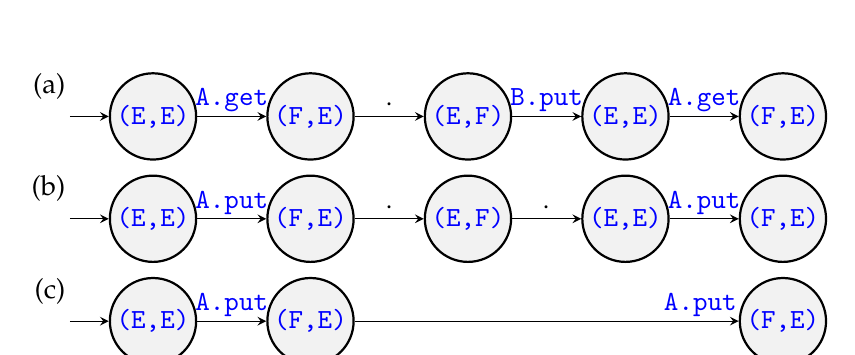
\begin{tikzpicture}[node distance=2cm, inner sep=0.5mm ]
	
	\node[state, initial, initial text=(a)\\\\] (qee) {\code{(E,E)}};
	\node[state, right of=qee] (qfe) {\code{(F,E)}};
	\node[state, right of=qfe] (qef) {\code{(E,F)}};
	\node[state, right of=qef] (qee2) {\code{(E,E)}};
	\node[state, right of=qee2] (qfe2) {\code{(F,E)}};
	
	\node[state, initial, below of=qee, yshift=7mm, initial text=(b)\\\\] (qee') {\code{(E,E)}};
	\node[state, right of=qee'] (qfe') {\code{(F,E)}};
	\node[state, right of=qfe'] (qef') {\code{(E,F)}};
	\node[state, right of=qef'] (qee2') {\code{(E,E)}};
	\node[state, right of=qee2'] (qfe2') {\code{(F,E)}};
	
	\node[state, initial, below of=qee', yshift=7mm, initial text=(c)\\\\] (qee'') {\code{(E,E)}};
	\node[state, below of=qfe', yshift=7mm] (qfe'') {\code{(F,E)}};
	\node[state, below of=qfe2', yshift=7mm] (qfe2'') {\code{(F,E)}};
	
	\draw
	(qee) edge[above] node{\code{A.get}} (qfe)
	(qfe) edge[above] node{$\cdot$} (qef)
	(qef) edge[above] node{\code{B.put}} (qee2)
	(qee2) edge[above] node{\code{A.get}} (qfe2)
	
	(qee') edge[above] node{\code{A.put}} (qfe')
	(qfe') edge[above] node{$\cdot$} (qef')
	(qef') edge[above] node{$\cdot$} (qee2')
	(qee2') edge[above] node{\code{A.put}} (qfe2')
	
	
	(qee'') edge[above] node{\code{A.put}} (qfe'')
	(qfe'') edge[above] node[pos=0.9]{\code{A.put}} (qfe2'')
	;
	\end{tikzpicture}
	\caption[RBAs in lockstep with and without normalization.]{Rules being applied to walk three RBAs in lockstep, with time horizontally, showing the (simplified) configurations traversed, and annotating rules by showing which port actions they involve.\\(a) RBA of protocol \textit{fifo2}. (b) RBA of \textit{fifo2} projected onto port set $\{A\}$. (c) RBA of \textit{fifo2} projected onto port set $\{A\}$ and normalized to remove silent rules.}
	\label{fig:path_sim}
\end{figure}



\begin{listing}[ht]
	\inputminted[]{rust}{normalize.rs}
	\caption[Normalization procedure Rusty-pseudocode.]{Normalization procedure, expressed in (simplified) Rust code. In a nutshell: while one exists, an arbitrary silent rule $x$ is removed, and the list of rules is extended with composed rules $x\cdot{}y$ such that $y$ is another rule.}
	\label{listing:normalize}
\end{listing}

The final normalization procedure is given in Listing~\ref{listing:normalize} in the form of simplified Rust code. It works intuitively for the most part: silent rules are removed, and new rules are added to retain their contribution of moving the RBA through configuration space. The function \code{normalize} ensures that the returned rule set is in the same configuration as the protocol after matching a non-silent, but the configuration is allowed to `lag behind' while the protocol performs rules which it considers to be silent. New rules must be added to `catch up' to the protocol after any such sequence of silent rules. The procedure does this by building these \textit{composed} rules from front to back, ie. replacing every silent rule $x$ with a \textit{set} of rules $x\cdot{}y$, where $y$ is any other rule. Once completed, the RBA may contain rules that are subject to \textit{simplification}. For example, \{$m=*\wedge{}n=*$, $m\neq{}*\wedge{}n=*$\} can be represented by only $n=*$.

The normalization algorithm is \textbf{correct} as clearly it does not have silent rules once it returns (\code{not\_silent} containing zero silent rules is invariant). Observe that for each silent rule removed, it does not consider composing with \textit{itself}. The immediate result is that the algorithm never inserts some rule $x\cdot{}x$ for silent rule $x$. This is not a problem, as all \textit{silent} rules of our approximated RBAs are \textit{idempotent} with respect to their impact on the configuration. The algorithm is able to take for granted that the result any \textit{chain} of silent rules $x\cdot{}x\cdot{}x\cdot{}...$ is covered by considering $x$ itself. Furthermore, the incremental removal of rules prohibits the creation of any silent cycles at all. This is due to the reasoning above being extended to any sequences also. (TODO PUMPING LEMMA).


The normalization algorithm is \textbf{terminating}. It consists of finitely many \textit{algorithm steps} in which the RBA $A$ is replaced by RBA $B=(A \setminus{}\{r\}) \cup{} \{r\cdot{}x | r\in{} A\setminus{}\{x\} \wedge{} composable(x,r)\}$ for some silent rule $x \in{} A$. Initially, $A$ is the input RBA with silent rules. The algorithm terminates, returning $B$ when $A$ is replaced by $B$ where $B$ has no silent rules. Let $P(x)$ be the set of \textit{acyclic paths} through RBA $x$'s configuration space. Observe that initially, $P(A)$ is finite. It suffices to show that in each algorithm round, $|P(A)|$ strictly decreases. Within a round, for every `added' $p$ in $P(B)\setminus{}P(A)$, $p$ contains a rule $m\cdot{}n$ such that there exists $p'$ in $P(A)\setminus{}P(B)$ identical to $p$ but with a 2-long sequence of rules $m, n$ in the place of $x$. From this we know that $|P(A)| \geq |P(B)|$. However, the 1-long path of $x$ itself is clearly in $P(A)\setminus{} P(B)$. Thus, $|P(A)| > |P(B)|$. \textsc{qed}.

To demonstrate the normalization procedure, Table~\ref{tab:fifo2_rbf_tsa_norm} shows the result of projecting the \textit{fifo2} connector's RBF onto port set $\{A,B\}$ and normalizing. The two additional rules can be understood to `cover' the behavior lost as a result of omitting the silent rule 1 from the original~RBF.


\begin{table}
	\centering
	\begin{tabular}{l|ll|}
		rule & guard & assignment \\
		\hline
		0 & $m_0=*$ & $\gapwedge{}m_0'=d_A$\\
		2 & $m_1\neq{}*$ & $\gapwedge{}d_B=m_1\gapwedge{}m_1'=*$ \\
		\hline
		$1\cdot{}0$ & $m_0\neq{}*\wedge{}m_1=*$ & $\gapwedge{}m_0'=d_A\wedge{}m_1'=m_0$ \\
		$1\cdot{}2$ & $m_0\neq{}*\wedge{}m_1=*$ & $\gapwedge{}m_0'=*$ \\
		\hline
	\end{tabular}
	\caption[RBF of fifo2 connector, projected and normalized.]{RBF of the \textit{fifo2} protocol, projected onto port set $\{A,B\}$ and normalized. Rules 0 and 2 are retained from Table~\ref{tab:fifo2_rbf_tsa}, and new rules $1\cdot{}0$ and $1\cdot{}2$ are composed of rules from the original RBF.}
	\label{tab:fifo2_rbf_tsa_norm}
\end{table}


\subsection{User-Defined Protocol Simplification}
\label{sec:user_defined_simplification}
Recall, the purpose of a governor is to preserve a system's \textit{liveness}.
They do this by ensuring that their governed compute component performs port operations that allow the interfacing protocol (and the system around it) to progress. 
Governors do this by enforcing that their compute component's implementation \textit{covers} each possible transition with code that performs the required task, and ensuring it is chosen correctly in accordance with the wishes of the protocol. Section~\ref{sec:rule_consensus} explains how our type-state automaton represents this by each configuration requiring the definition of a \textit{set} of transitions, one for each action. We say the implementation `covers' each of these cases by defining the component's behavior in each cases, including the invocation of the relevant port operation.

An overzealous governor which requires to cover \textit{additional} (unnecessary) cases would still serve its purpose. In effect, such a governor would enforce adherence to some \textit{other}, more permissive protocol. However, liberty of the protocol means responsibility to the compute-component: the more the protocol \textit{might do}, the more the compute-component \textit{must consider doing}. There is incentive for governors to do this: permissive protocols are simpler to enforce.

This conservatism becomes a problem when it infringes on the component's ability to express its behavior as intended. Consider the example of a compute-component~$X$ that forwards values from its input port~$A$ to its output port~$B$. Perhaps this component is used in a pipeline as intended such that the component is involved in an endlessly-alternating sequence, represented by regular expression~$(AB)^*$. Perhaps there is a sensible way for $X$ to implement the more permissive protocol which permits~$B$ firings to be omitted, expressed $(A(B|\lambda{}))^*$. $P$ has no problem discarding values input from $A$. However, if the governor takes it a step further such that `anything goes' (expressed $(A|B)^*$), $X$~cannot meaningfully represent its work. How on earth can it forward a message to $B$ before receiving it on~$A$? Not even clairvoyance can help; what if $A$ never fires at all? This is how the user would experience the problem of a governor infringing on the component's own behavior; in a sense,~$P$ has a protocol of its own which must be preserved on its interface ports which the governor violates.



\begin{table}
	\centering
	\begin{tabular}{l|ll}
		rule & guard & assignment \\
		\hline
		0 & $m_0=*$
		& $\gapwedge{}m_0'=d_A$\\
		1 & $m_0\neq{}*\wedge{}m_1=*$
		& $\gapwedge{}m_1'=d_A\wedge{}m_0'=*$\\
		2 & $m_0=m_1\neq{}*\wedge{}m_2=*$
		& $\gapwedge{}m_2'=d_A\wedge{}m_0'=m_1'=*$\\
		3 & $m_0=m_1=m_2\neq{}*$
		& $\gapwedge{}d_B=m_0\wedge{}m_0'=m_1'=m_2'=*$\\
		\hline
	\end{tabular}
	\caption{RBF of the \textit{a7b1} connector, which is characterized by cycling through a predictable sequence of period~8, where~$A$ inputs seven times and~$B$ outputs once. It works by encoding its configuration in an 8-long cycle as a three-bit integer using the fullness of memory cells $m_{0-2}$.}
	\label{tab:counting_rbf}
\end{table}

Nevertheless, there is value in providing a compute-component with a simplified (permissive) view of the protocol where possible. As a motivating example, consider the \textit{a7b1} connector, given as RBF in Table~\ref{tab:counting_rbf}. This connector uses the fullness of three memory cells to count in binary from zero to seven (using the binary alphabet of memory cell states $\{\text{\code{E}}, \text{\code{F}}\}$), and cycling back again to zero. Configurations in this cycle are distinguished by specifying different behaviors on~$A$ and~$B$. Here, the projection and normalization of the protocol's RBF is trivial, as no rules are silent. Without the ability to simplify, the~$Y$ must be implemented such that it corresponds exactly with the protocol's (predictable) walk through its approximated configuration space, given in Figure~\ref{fig:counter_RBAs}. As all states are distinguishable, so too are their corresponding \textit{state types} distinct. Now consider this protocol interfacing with some compute-component~$Y$, which is always ready to consume and emit some data element~\textit{Q}. Without simplification, the resulting governor would require that the traversal through configuration space be spelled out; the user would be forced to distinguish these states, even though~$Y$ has no need for this specificity. Most likely, the resulting implementation will be repetitive and verbose, if the behavior is the same for configurations \code{(EEE)}, \code{(EEF)}, et cetera.

\begin{figure}[ht]
	\centering
	\footnotesize
	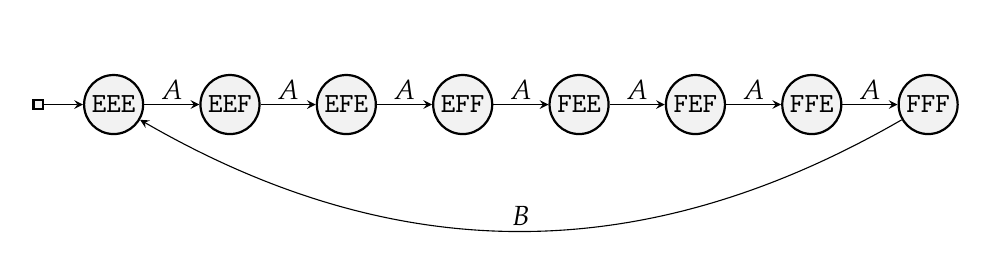
\begin{tikzpicture}
	[ inner sep=0.6mm ]
	\matrix (m) [ matrix of nodes, row sep=0.5cm, column sep = 0.7cm, 
	nodes = {anchor=center,circle, draw=black, thick, fill=gray!10},] {
		\node(m0)[initial]{\texttt{EEE}}; & \node(m1){\texttt{EEF}}; & \node(m2){\texttt{EFE}}; & \node(m3){\texttt{EFF}}; & \node(m4){\texttt{FEE}}; & \node(m5){\texttt{FEF}}; & \node(m6){\texttt{FFE}}; & \node(m7){\texttt{FFF}};\\
	};
	\draw
	(m0) edge[above] node{$A$} (m1)
	(m1) edge[above] node{$A$} (m2)
	(m2) edge[above] node{$A$} (m3)
	(m3) edge[above] node{$A$} (m4)
	(m4) edge[above] node{$A$} (m5)
	(m5) edge[above] node{$A$} (m6)
	(m6) edge[above] node{$A$} (m7)
	(m7) edge[bend left, above] node{$B$} (m0)
	;
	\end{tikzpicture}
	\caption[Configuration space of the a7b1 connector.]{Rules transitioning through configuration space of approximated RBAs for \textit{a7b1} connector, with states named after the `count' the three memory cells represent in base~2 (in binary alphabet $\{\text{\code{E}}, \text{\code{F}}\}$). Here, the normalization procedure with interface set~$\{A,B\}$ is trivial as no transitions are silent.}
	\label{fig:counter_RBAs}
\end{figure}

Our solution to this problem is to introduce a third type for representing the state of a memory cell which may be \textit{either} full or empty:~\code{Unknown} (abbreviated as~\code{U}). Rather than corresponding to a specific configuration of the (approximated) RBA, the governor now reasons about the \textit{set} of states which the protocol may be in. For example, type \code{(UUE)} encapsulates all the concrete configuration types $\{\text{\code{(EEE)}}, \text{\code{(EFE)}}, \text{\code{(FEE)}}, \text{\code{(FFE)}}\}$, and is liable to covering the \textit{union} of the rules applicable to any of those states. In this manner, it is safe for the programmer to arbitrarily `forget' the state of a memory cell, replacing its element in the tuple type with~\code{U}. To be clear, \code{U} is not special as far as Rust is concerned; we have changed to a ternary alphabet for representing memory cells in types. However, \code{U} does not correspond to any real configuration that memory cells are ever `really' in at runtime; they are always either empty or full. \code{U} is a stand-in for an empty \textit{or} full memory variable, an abstraction in which the protocol is not (explicitly) involved.
With this tool in their belt, the implementation of the compute component is able to arbitrarily \textit{unify} the state-types of multiple branches. Our example component~$Y$ above is able to implement its behavior to the satisfaction of its governor with transitions through configuration space in Figure~\ref{fig:weakening}. This weakening can be communicated quite ergonomically, resulting in something very close to what the user would implement themselves: a single loop where the four rules (numbered 0-3) may be applied to configuration type~\code{(UUU)}, each resulting again in~\code{(UUU)}.


\begin{figure}[ht]
	\centering
	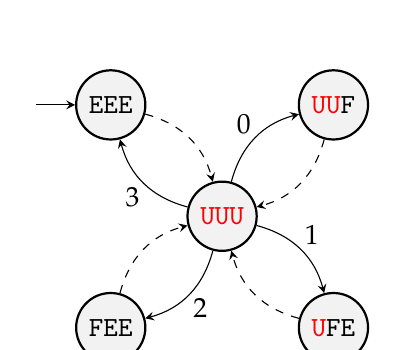
\begin{tikzpicture}[node distance=2cm, inner sep=0.5mm ]
	\node[state, initial]      (q000) {\texttt{EEE}};
	\node[state, below right of=q000] (q???) {\texttt{\textcolor{red}{UUU}}};
	\node[state, above right of=q???] (q??1) {\texttt{\textcolor{red}{UU}F}};
	\node[state, below right of=q???] (q?10) {\texttt{\textcolor{red}{U}FE}};
	\node[state, below left of=q???] (q100) {\texttt{FEE}};
	\draw
%	weakenings
	(q000) edge[dashed, bend left] node{} (q???)
	(q??1) edge[dashed, bend left] node{} (q???)
	(q?10) edge[dashed, bend left] node{} (q???)
	(q100) edge[dashed, bend left] node{} (q???)

%	actual transitions
	(q???) edge[above left, bend left] node{0} (q??1)
	(q???) edge[above right, bend left] node{1} (q?10)
	(q???) edge[below right, bend left] node{2} (q100)
	(q???) edge[below left, bend left] node{3} (q000)
	;
	\end{tikzpicture}
	\caption[Traversed configuration space for a7b1 connector using weakening.]{Rules transitioning between configurations of the \textit{a7b1} connector shown in Figure~\ref{fig:counter_RBAs}. Here, the user employs \textit{weakening} to convert (dashed arrows) state tokens to configurations to the configuration-set `???' containing \textit{all} concrete configurations. RBA rules firing are shown with solid arrows, annotated with the rule name, corresponding to those given in Table~\ref{tab:counting_rbf}.}
	\label{fig:weakening}
\end{figure}



%How can the governor know which distinguishable states the compute components does not wish to distinguish? Our solution is to provide a means for \textit{unifying} 
%We cannot know a priori which distinguishable states the compute component \textit{wishes} to distinguish. Ideally, the user has an ergonomic means of making this choice themselves. Our solution introduces a means for 
%
%
%We currently consider memory variables of the binary domain, ie.\ each is either in state~\code{Full} or~\code{Empty}. We introduce a third state with type \code{Unknown}. Conceptually, configurations with \code{Unknown}-state memory cells represent protocol configurations where each is either concretely full or empty, ie.\ the governor `cannot remember'. 
%
%
%Section~\ref{sec:rule_consensus} describes how the Governor must already be prepared to handle configurations for which there are multiple possible \textit{next} transitions. By adding 
%
%As far as the compiler is concerned, \code{Unknown} is just another state, as distinct from \code{Empty} or \code{Full} as any other. Conceptually, we use \code{Unknown} to represent th
%
%type for a new state memory cells can be in to supplement existing types \code{Empty} and~\code{Full}:~\code{Unknown}. A type-state with memory cells in an \textit{unknown} state is obliged to cover the \textit{union} of all its concrete possibilities. For example, \code{(Empty, Unknown)} may result in any states either \code{(Empty, Empty)} or \code{(Empty, Full)} may result in. With this definition, it is perfectly correct for a state-type to be `weakened', converting it into a new state-type, identical but with any of its tuple-elemets replaced by \code{Unknown}. In a sense, this approach has type-states no longer corresponding with configurations 1-to-1, but rather, each type-state encodes a simple predicate such that it represents a \textit{set} of configurations. For example, \code{(Unknown, Unknown)} represents \textit{any} configuration (of an RBA with two memory cells). Conceptually, this change has no influence on the way a governor computes which rules are applicable next, but the programmer is empowered with the ability to trade \textit{specificity} for \textit{brevity} in their compute-component implementations. Figure~\ref{fig:weakening} shows an example of how the programmer may choose to traverse their configuration space for the same connector as in the example above. In this case, using \textit{weakening} does not reduce the number of type-states encountered in the implementation; this is only the result of (a) the original RBA not being very complicated, and (b) the choice to only \textit{partially} weaken some states (It is also possible to weaken everything to \code{(Unknown, Unknown, Unknown)} and then match all rules).
%
%
%\begin{figure}[ht]
%	\centering
%	\begin{tikzpicture}[node distance=2cm, inner sep=0.5mm ]
%	\node[state, initial]      (q000) {\texttt{000}};
%	\node[state, right of=qee] (q??0) {\texttt{\textcolor{red}{??}0}};
%	\node[state, right of=q??0] (q??1) {\texttt{\textcolor{red}{??}1}};
%	\node[state, below of=q??1] (q?11) {\texttt{\textcolor{red}{?}11}};
%	\node[state, right of=q??1] (q101) {\texttt{101}};
%	\draw
%	(q000) edge[dashed] node{} (q??0)
%	(q??0) edge[above] node{0} (q??1)
%	(q??1) edge[below, bend left] node{3} (q000)
%	
%	(q??1) edge[left, bend right] node{$1\cdot{}0$} (q?11)
%	(q?11) edge[dashed] node{} (q??1)
%	
%	(q??1) edge[below, bend right] node{$2\cdot{}0$} (q101)
%	(q101) edge[dashed] node{} (q??1)
%	;
%	\end{tikzpicture}
%	\caption{Rules transitioning between configurations of the \textit{8-count cycle} connector in Figure~\ref{fig:counter_RBAs}. Here, the user employs \textit{weakening} to convert (dashed arrows) state tokens to configurations with \textit{unknown} memory cell states. RBA rules firing are shown with solid arrows, annotated with the rule name, corresponding to those given in Table~\ref{tab:counting_rbf}. Note that not all possible weakenings are shown, only an example set that covers all rules.}
%	\label{fig:weakening}
%\end{figure}


\subsection{Match Syntax Sugar}
Section~\ref{sec:rule_consensus} explains how the set of transitions to be covered by a configuration type can be represented in Rust's type system as a tail-recursive list. This alleviates the problem of having to explicitly enumerate the needed sets each as their own enumeration type. This is necessary, as the upper-bound\footnote{Many factors reduce this number drastically in practice. For example, state-sets are usually not large because they are only ever encountered when reached by \textit{transitions} from some state.} of state sets is $2^{3^M}$, where $M$ is the number of memory cells\footnote{The number of unique state sets is $2^S$, where $S$ is the number of configurations (automaton state types). This, in turn is $3^M$, as each memory cell's state is represented by a type in $\{\text{\code{E}}, \text{\code{F}}, \text{\code{U}}\}.$}; suffice it to say, it is \textit{a~lot}.
Unfortunately, these are not natively-supported enumeration types, and thus cannot be \textit{matched} as is idiomatic in the Rust language. However, Rust has extensive support for abstract syntax tree \textit{macros}, allowing us to have the best of both worlds; the user interacts with \code{StateSet} types by using a match-like macro which enumerates the branches, but there is no need for concrete \code{enum} classes to be defined for all the conceivable combinations. Figure~\ref{listing:sugar} gives an example of how these cases compare to one another.


\begin{listing}[ht]
	\centering
	\inputminted{rust}{sugar.rs}
	\caption[Example of mimicing enum matching with a sugaring macro.]{Example of three methods for matching a \textit{state set}, representing a sum type of three variant types simplified here to \code{X}, \code{Y} and \code{Z}. First, \code{match\_standard} shows how this is done in idiomatic Rust, requiring an enum type \code{StateSetXyz} be explicitly defined. \code{match\_recursive} shows how the same state set represented by a tail-recursive \code{StateSet} type can be similarly matched by exhaustively `unzipping' head elements using a function \code{match\_head}. finally, \code{match\_macro} functions identically to the second case, but relies on a sugaring macro \code{match\_set} to mimic the syntax of Rust's \code{match} statement, seen in the first function.}
	\label{listing:sugar}
\end{listing}
\chapter{Benchmarking}
\section{Goal}
\section{Experimental Setup}
\section{Results}
\section{Observations}

\part{Reflection}
\chapter{Discussion}
\label{sec:discussion}
\section{Future Work}
\hl{TODO short intro}
\subsection{Imperative Form Compiler}
Chapters~\ref{sec:imperative_form} and~\ref{sec:protocol_runtime} explain how the Reo-rs runtime makes use of a lightweight interpreter to bring life to our protocol objects at runtime according to the appropriate specification. This \textit{commandification} pattern has its advantages; namely, protocol behavior is alterable at runtime by manipulating the interpreted data. However, this flexibility does not come for free. The interpretation steps incur overhead both to the protocol construction procedure, and more importantly, to the work of \textit{port operations}. Fortunately, our \textit{imperative form} does not necessitate the use of an interpreter. Future work could investigate replacing the \code{build} procedure of Reo-rs with another compilation step such that the behavior is represented in native, directly-executable Rust. 

Futhermore, future work might investigate the use of custom \textit{domain specific languages} for compiling imperative form in a manner that it performs the same checking as in \code{build} \textit{statically}. the obvious means of doing this is to build a compiler from scratch. However, other options exist that can make better use of existing tools. For example, Rust's \textit{procedural macros} allow the programmer to define arbitrary transformations of Rust's \textit{abstract syntax trees} during compilation. Essentially, one is able to invoke arbitrary, pre-compiled Rust code \textit{inside} the user's Rust compiler itself. In this manner, one can embed the needed domain-specific language into the Rust compiler itself.

\subsection{Distributed Components}
\hl{TODO refer to Reowolf. talk about how protocols can become distributed by partitioning their memory space. problem is complex. involves consensus. refer to reowolf project. refer to farhad's and sung's previous work}
\subsection{Imperative Branching}
\hl{as propositional formulas can be converted to DNF (with disjunctions on the outermost layer), so too can imperative form rules be split over OR branches into new rules (EXAMPLE). This idea can be taken to the extreme: splitting over the elements of the data domain and once again enumerating the transition space, resulting in something with the most degenerate RBAs possible with an explosion in rules. In some cases, moving in this direction is desirable, as it has the effect of making the rule GUARDS do all of the checking; as seen earlier, boolean guarded variables can be efficiently checked in bulk. THe extreme of the spectrum is unlikely to be more efficient: the same transform values will be computed and discarded repeatedly, and as the number of boolean variables increases, at some point even batch-computing them falls behind. Future work could investigate this balance between a small number of rules, and determinisms in rules.}
\subsection{Runtime Governors}
\hl{TODO}
more abstract suggestion. runtime governers. makes it possible to use them without affine types. eg in C

\subsection{Further Runtime Optimization}
\hl{Didn't implement everything for variious reasosn but lots is possible}
\begin{enumerate}
	\item simplify or remove predicates based on implicit information if rules have a KNOWN ordering. EG:: before [if P, if not P]. after [if P, true]
	\item stuffed pointers for data types with representations no larger than ptr size. no need for allocator. complicates the refcounter mechanism
	\item imperative form preprocessing. some redundancy exists in how you can represent things. eg: MemSwap sometimes can be achieed just by reorganizing your movements. more examples: pruning check subtries of tautologies and contradictions. this can happen in either reo or reo-rs
\end{enumerate}
\subsection{Avoid Lock Re-Entry}
\hl{when you empty a memcell you need to coordinate again. would be nice if we can avoid locking a second time by either detecting when we know it will be unnecessary or just some mechanism to delegate the work}
\subsection{Runtime Reconfiguration}
\hl{our protocol is data. we can change it and change its behavior. care must be taken because you are reconfiguring the structure laid out for speed}
\section{Conclusion}
\hl{TODO}


\bibliographystyle{alpha}
\bibliography{references}

\end{document}